\documentclass[10pt]{article}
\usepackage{../pplmanual}
%%% Commonly Needed packages
\usepackage{graphicx,color,calc}
\usepackage{fancyvrb}
\usepackage{makeidx}
\usepackage{alltt}
\usepackage{html}
\usepackage{hyphenat}
\usepackage{listings}
\usepackage{xspace} %<- creates problems with other hyperlink packages like "html"
\usepackage{hyperref}
\hypersetup{
    colorlinks,%
    citecolor=black,%
    filecolor=black,%
    linkcolor=black,%
    urlcolor=magenta
}


%%% Commands for uniform looks of C++, Charm++, and Projections
\newcommand{\CC}{C\hbox{++}\xspace}
\newcommand{\emCC}{C\hbox{\em++}\xspace}
\newcommand{\charmpp}{Charm++\xspace}
\newcommand{\charm}{Charm++\xspace}
\newcommand{\charmc}{\texttt{charmc}\xspace}
\newcommand{\projections}{\textrm{Projections}\xspace}
\newcommand{\converse}{Converse\xspace}
\newcommand{\ampi}{\textup{AMPI}\xspace}
\newcommand{\tempo}{\textsc{TeMPO}\xspace}
\newcommand{\irecv}{\textsl{iRecv}\xspace}
\newcommand{\sdag}{\textsl{Structured Dagger}\xspace}
\newcommand{\jade}{Jade\xspace}
\newcommand{\ci}{\emph{ci}\xspace}

%%% Commands to produce margin symbols
\newcommand{\new}{\marginpar{\fbox{\bf$\mathcal{NEW}$}}}
\newcommand{\important}{\marginpar{\fbox{\bf\Huge !}}}
\newcommand{\experimental}{\marginpar{\fbox{\bf\Huge $\beta$}}}

%%% Commands for manual elements
\newcommand{\zap}[1]{ }
\newcommand{\function}[1]{{\noindent{\textsf{#1}}\\}}
\newcommand{\cmd}[1]{{\noindent{\textsf{#1}}\\}}
\newcommand{\args}[1]{\hspace*{2em}{\texttt{#1}}\\}
\newcommand{\prototype}[1]{\vspace{0.2in}\index{#1}}
\newcommand{\param}[1]{{\texttt{#1}}}
\newcommand{\kw}[1]{{\nohyphens{\textsf{#1}}\index{#1}}}
\newcommand{\uw}[1]{#1}
\newcommand{\desc}[1]{\indent{#1}}
\newcommand{\note}[1]{(\textbf{Note:} #1)}
\newcommand{\term}[1]{{\bf #1}\index{#1}}

% Explicitly state that part numbering uses uppercase roman numerals
% This is just to keep latex2html from barfing and causing a filename
% collision between part II and chapter 2 etc. This will work as long
% as we don't have an appendix section 9 (which would be alphabetized
% to I (and again conflict with part 1).
\renewcommand{\thepart}{\Roman{part}}

\newcommand{\gitweb}[2]{http://charm.cs.illinois.edu/cgi-bin/gitweb2.cgi?p=charm.git;hb=HEAD;a=#1;f=#2}

\newcommand{\gitwebref}[3]{\href{\gitweb{#1}{#2/charm\%2B\%2B/#3}}{\tt #2/charm++/#3}}
\newcommand{\examplereffile}[1]{\gitwebref{blob}{examples}{#1}}
\newcommand{\examplerefdir}[1]{\gitwebref{tree}{examples}{#1}}
\newcommand{\testreffile}[1]{\gitwebref{blob}{tests}{#1}}
\newcommand{\testrefdir}[1]{\gitwebref{tree}{tests}{#1}}

\begin{htmlonly}
\renewcommand{\examplereffile}[1]{\texttt{\emph{examples/charm++/#1}}}
\renewcommand{\examplerefdir}[1]{\texttt{examples/charm++/#1}}
\renewcommand{\testreffile}[1]{\texttt{\emph{tests/charm++/#1}}}
\renewcommand{\testrefdir}[1]{\texttt{tests/charm++/#1}}
\end{htmlonly}
\makeindex


\makeindex

\title{\charmpp\\ Finite Element Method (FEM) Framework\\ Manual}
\version{1.2}
\credits{
Initial version of \charmpp{} FEM Framework was developed
by Milind Bhandarkar with inputs from Timothy Hinrichs and Karthikeyan
Mahesh. The current version is almost completely rewritten by
Orion Lawlor. The most recent version is being called by the name ParFUM. 
ParFUM is short for Parallel Framework for Unstructured Meshes. 
This version has been mostly written by Nilesh Choudhury, Terry Wilmarth,
Sayantan Chakravorty and Issac Dooley.}

\begin{document}

\maketitle

\section{Introduction}

The Finite Element Method (FEM) approach is used in many engineering
applications with irregular domains, from elastic deformation problems to
crack propagation to fluid flow.  \charmpp{} is a free message-passing parallel
runtime system for machines from clusters of workstations to tightly-coupled
SMPs.  The \charmpp{} FEM framework allows you to write a parallel FEM program,
in C or Fortran 90, that closely resembles a serial version but includes
a few framework calls.

Using the FEM framework also allows you to take advantage of all the
features of \charmpp, including run-time load balancing,  performance
monitoring and visualization, and checkpoint/restart, with no additional
effort. The FEM framework also combines naturally with other \charmpp
frameworks built on TCHARM.

The FEM framework has been undergoing a wave of recent improvements. A choice to rename the new version ParFUM has been adopted.ParFUM is short for Parallel Framework for Unstructured Meshes. Section \ref{sec:ParFUM} describes some of the new features included in ParFUM that were not present in FEM.


\subsection{Philosophy}

The \charmpp{} FEM framework is designed to be flexible, in that it
provided a few very general operations, such as loading and partitioning 
a ``mesh.''  
In describing these operations, we draw on examples from structural analysis,
but in fact the same calls can be used for other applications, including
fluid dynamics or partial differential equations solvers, or
even general-purpose graph manipulation.

For example, the FEM framework does not specify the number of spatial
dimensions.  Node locations are treated as just another kind of node data,
with no restrictions on the number of data items.
This allows the FEM framework to work with problems having any number 
of spatial dimensions.


\subsection{Terminology}
\label{sec:terminology}

A FEM program manipulates elements and nodes. An \term{element} is a portion of
the problem domain, also known as a cell, and is typically some simple shape 
like a triangle, square, or hexagon in 2D; or tetrahedron or rectangular solid in 3D.  
A \term{node} is a point in the domain, and is often the vertex of several elements.  
Together, the elements and nodes form a \term{mesh}, which is the 
central data structure in the FEM framework.

An element knows which nodes surround it via the element's
\term{connectivity table}, which lists the nodes adjacent to each element.

\begin{figure}[h]
\begin{center}
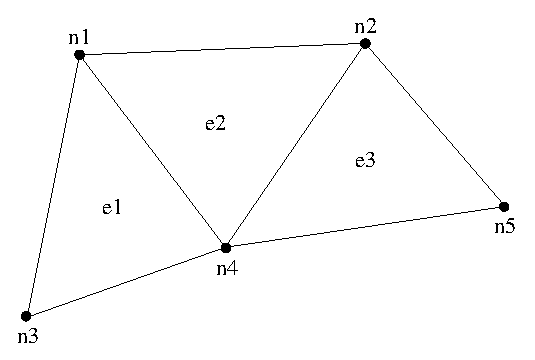
\includegraphics[width=4in]{fig/simple_mesh}
\end{center}
\caption{3-element, 5 node mesh.}
\label{fig:simplemesh}
\end{figure}

\begin{table}[h]
\begin{center}
\begin{tabular}{||l||l|l|l||}\hline
Element & \multicolumn{3}{c||}{Adjacent Nodes} \\\hline
e1 & n1 & n3 & n4 \\
e2 & n1 & n2 & n4 \\
e3 & n2 & n4 & n5 \\
\hline
\end{tabular}
\end{center}
\caption{Connectivity table for mesh in figure~\ref{fig:simplemesh}.}
\label{table:simplemesh}
\end{table}

A typical FEM program performs some element-by-element calculations which
update adjacent node values; then some node-by-node calculations.  For
example, a material dynamics program has the structure:

\begin{alltt}
     time loop
          element loop-- Element deformation applies forces to
          surrounding nodes
          node loop-- Forces and boundary conditions change node
          positions
     end time loop
\end{alltt}

We can parallelize such FEM programs by partitioning the serial mesh
elements into several smaller meshes, or \term{chunks}.  There is normally
at least one chunk per processor; and often even more.  During partitioning, 
we give nodes and elements new, \term{local} numbers within that chunk.
In the figure below, we have partitioned the mesh above into two chunks, A and B.

\begin{figure}[h]
\begin{center}
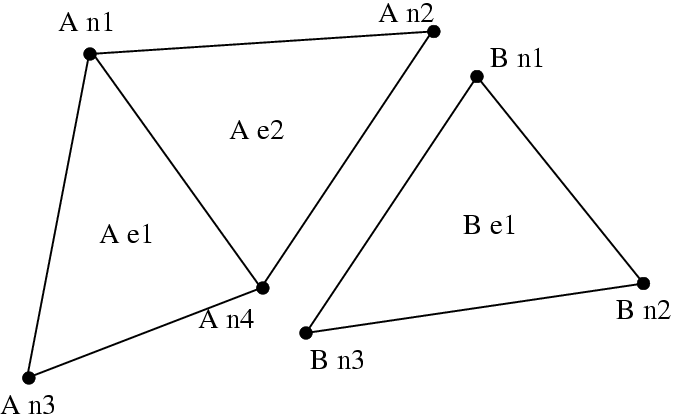
\includegraphics[width=4in]{fig/partitioned_mesh}
\end{center}
\caption{Partitioned mesh.}
\label{fig:partitionedmesh}
\end{figure}

\begin{table}[hh]
\begin{center}
\begin{tabular}{||l||l|l|l||}\hline
Element & \multicolumn{3}{c||}{Adjacent Nodes} \\\hline
e1 & n1 & n3 & n4 \\
e2 & n1 & n2 & n4 \\
\hline
\end{tabular}
\end{center}
\caption{Connectivity table for chunk A in figure~\ref{fig:partitionedmesh}.}
\label{table:chunkA}
\end{table}

\begin{table}[hh]
\begin{center}
\begin{tabular}{||l||l|l|l||}\hline
Element & \multicolumn{3}{c||}{Adjacent Nodes}\\\hline
e1 & n1 & n2 & n3 \\
\hline
\end{tabular}
\end{center}
\caption{Connectivity table for chunk B in figure~\ref{fig:partitionedmesh}.}
\label{table:chunkB}
\end{table}

Note that chunk A's node n2 and B's node n1 were actually the same node in
the original mesh-- partitioning split this single node into two shared
copies (one on each chunk).  However, since adding forces is associative, we
can handle shared nodes by computing the forces normally (ignoring the
existence of the other chunk), then adding both chunks' net force for the
shared node together.  This ``node update'' will give us the same resulting
force on each shared node as we would get without partitioning, thus the
same positions, thus the same final result.  

For example, under hydrostatic pressure, each chunk might compute a local
net force vector for its nodes as shown in Figure~\ref{fig:forcedecomp}
(a).  After adding forces across chunks, we have the consistent global forces
shown in Figure~\ref{fig:forcedecomp} (b).

\begin{figure}[h]
\begin{center}
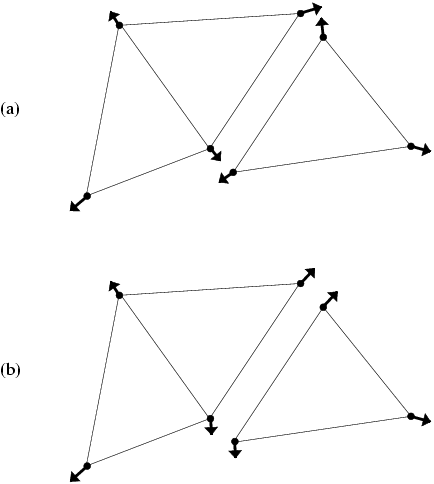
\includegraphics[height=3in]{fig/forcedecomp}
\end{center}
\caption{A force calculation decomposed across chunks: (a) before update
(b) after updating forces across nodes.}
\label{fig:forcedecomp}
\end{figure}

Hence, each chunk's time loop has the structure:

\begin{alltt}
     chunk time loop
          element loop-- Element deformation applies forces to
          surrounding nodes
          <update forces on shared nodes>
          node loop-- Forces and boundary conditions change node
          positions
     end time loop
\end{alltt}

This is exactly the form of the time loop for a \charmpp{} FEM framework
program.  The framework will accept a serial mesh, partition it, distribute
the chunks to each processor, then you run your time loop to perform
analysis and communication.


\subsection{Structure of a Classic FEM Framework Program}

A classic FEM framework program consists of two subroutines: 
\kw{init()} and \kw{driver()}.
\kw{init()} is called by the FEM framework
only on the first processor -- this routine typically does specialized I/O,
startup and shutdown tasks.  \kw{driver()} is called for every chunk on every
processor, and does the main work of the program.  In the language of the
TCHARM manual, \kw{init()} runs in the serial context, 
and \kw{driver()} runs in the parallel context.

\begin{alltt}
     subroutine init
          read the serial mesh and configuration data
     end subroutine
/* after init, the FEM framework partitions the mesh */
     subroutine driver
          get local mesh chunk
          time loop
               FEM computations
               communicate boundary conditions
               more FEM computations
          end time loop
     end subroutine
\end{alltt}

In this mode, the FEM framework sets up a default writing
mesh during \kw{init()}, partitions the mesh after \kw{init()},
and sets up the partitioned mesh as the default reading mesh 
during \kw{driver()}. 


\subsection{Structure of an AMPI FEM Framework Program}

In addition to the classic init/driver structure above,
you can write an FEM framework program using the MPI style.
This is a more general, more flexible method of running
the program, but it is more complicated than the classic mode.
All FEM framework calls are available in either mode.

\begin{alltt}
   main program
      MPI_Init
      FEM_Init(MPI_COMM_WORLD)
      if (I am master processor)
         read mesh
      partition mesh
      time loop
          FEM computations
          communicate boundary conditions
          more FEM computations
      end time loop
   end main program
\end{alltt}

In this mode, the FEM framework does not set a default
reading or writing mesh, and does no partitioning;
so you must use the FEM\_Mesh routines to create and 
partition your mesh.
See the AMPI manual for details on how to declare
the main routine.

The driver() portion of a classic FEM program
strongly resembles an MPI mode main routine---in fact, a classic
FEM program can even make MPI calls from its \kw{driver()} 
routine, because the FEM framework is implemented directly on
top of MPI.  

There is even a special shell script for collecting
up the FEM framework source code to build a non-Charm, 
MPI-only version of the FEM framework.
To build FEM in this manner, you first build Charm++ normally,
then run a script to collect up the neccessary source files
(the FEM framework, a small number of Charm configuration 
and utility files, and the METIS library),
and finally build the library using the usual MPI compiler 
commands:
\begin{alltt}
 > cd charm/
 > ./src/libs/ck-libs/fem/make_fem_alone.sh
 > cd fem_alone/
 > mpicc -I. -DFEM_ALONE=1 -c *.c *.C 
 > ar cr libfem_alone.a *.o
\end{alltt}
You will then have to build your application with the MPI
compilers, and manually point to this ``fem\_alone'' 
directory to find include files and the new FEM library.
A typical compiler invocation would be:
\begin{alltt}
 > mpif90 -I$HOME/charm/fem_alone -L$HOME/charm/fem_alone foo.f90 -lfem_alone -o foo
\end{alltt}
This ``standalone'', non-Charm++ method of building the 
FEM framework prevents the use of load balancing or the other
features of Charm++, so we do not recommend it for normal use.


\subsection{Compilation and Execution}

A FEM framework program is a \charmpp\ program, so you must begin by
downloading the latest source version of \charmpp\ from
{\tt http://charm.cs.uiuc.edu/}.  Build the source with 
{\tt ./build FEM version} or {\tt cd} into the build directory, 
{\tt version/tmp}, and type {\tt make FEM}.
To compile a FEM program, pass the {\tt -language fem} (for C) or 
{\tt -language femf} (for Fortran) option to {\tt charmc}.
You can also build using the ``fem\_alone'' mode described
at the end of the section above.

In a charm installation, see charm/version/pgms/charm++/fem/
for several example and test programs.

At runtime, a Charm++/FEM framework program accepts the following
options, in addition to all the usual Charm++ options described in 
the Charm++ ``Installation and Usage Manual''.

\begin{itemize}
\item {\tt +vp} $v$  

Create $v$ mesh chunks, or ``virtual processors''.
By default, the number of mesh chunks is equal to the number of 
physical processors (set with {\tt +p} $p$).


\item {\tt -write}

Skip \kw{driver()}.
After running \kw{init()} normally, the framework partitions the mesh, 
writes the mesh partitions to files, and exits.  As usual, the
{\tt +vp} $v$ option controls the number of mesh partitions.

This option is only used in the classic mode---MPI-style programs
are not affected.


\item {\tt -read}

Skip \kw{init()}.
The framework reads the partitioned input mesh from files
and calls \kw{driver()}.  Together with {\tt -write}, this option
allows you to separate out the mesh preparation and partitioning 
phase from the actual parallel solution run.

This can be useful, for example, if \kw{init()} requires more memory 
to hold the unpartitioned mesh than is available on one processor of 
the parallel machine.  To avoid this limitation, you can run the program
with {\tt -write} on a machine with a lot of memory to prepare the input
files, then copy the files and run with {\tt -read} on a machine with 
a lot of processors.

{\tt -read} can also be useful during debugging or performance tuning, 
by skipping the (potentially slow) mesh preparation phase.
This option is only used in the classic mode---MPI-style programs
are not affected.


\item {\tt +tcharm\_trace fem}

Give a diagnostic printout on every call into the FEM framework.
This can be useful for locating a sudden crash, or understanding
how the program and framework interact.  Because printing the 
diagnostics can slow a program down, use this option with care.

\end{itemize}


\section{FEM Framework API Reference}

Some of the routines in the FEM framework have different requirements or meanings
depending on where they are called from.  When a routine is described
as being ``called from driver'', this means it is called in the parallel
context---from \kw{driver()} itself, any subroutine called by \kw{driver()},
or from whatever routine is run by the FEM-attached TCHARM threads.
When a routine is described as being ``called from init'', this means it is 
called in the serial context---from \kw{init()} itself, from any subroutine
called from \kw{init()}, from a routine called by \kw{FEM\_Update\_mesh},
or from whatever TCHARM code executes before the \kw{FEM\_Attach}.


\subsection{Utility}

\prototype{FEM\_Num\_partitions}
\function{int FEM\_Num\_partitions();}
\function{INTEGER FUNCTION :: FEM\_Num\_partitions()}

     Return the number of mesh chunks in the current computation.  Can
     only be called from the driver routine.

\prototype{FEM\_My\_partitions}
\function{int FEM\_My\_partition();}
\function{INTEGER FUNCTION :: FEM\_My\_partition()}

     Return the number of the current chunk, from 0 to
     \kw{num\_partitions}-1.  Can only be called from the driver routine.

\prototype{FEM\_Timer}
\function{double FEM\_Timer();}
\function{DOUBLE PRECISION FUNCTION :: FEM\_Timer()}

     Return the current wall clock time, in seconds.  Resolution is
     machine-dependent, but is at worst 10ms.

\prototype{FEM\_Print\_partition}
\function{void FEM\_Print\_partition();}
\function{SUBROUTINE FEM\_Print\_partition()}

     Print a debugging representation of the current chunk's mesh.
     Prints the entire connectivity array, and data associated with
     each local node and element.

\prototype{FEM\_Print}
\function{void FEM\_Print(const char *str);}
\function{SUBROUTINE FEM\_Print(str)}
\args{CHARACTER*, INTENT(IN) :: str}

     Print the given string, with "[<chunk number>]" printed 
     before the text.  

     This routine is no longer required: you can now use 
     the usual printf, PRINT, or WRITE statements.


\section{Mesh Nodes and Elements}
\label{sec:entities}

These routines describe and retreive the finite element mesh for this
computation.  A \term{mesh}, from the framework's perspective, is a list of
elements, nodes, and other data that describes the computational domain.
The FEM framework provides extensive support for creating, manipulating,
and partitioning meshes. 

A \term{serial mesh} consists of a single large piece.  It's usually
easiest to read and write serial meshes to existing, non-parallel file formats,
and it can be easier to manipulate serial meshes.  By contrast, a 
\term{parallel mesh} consists
of several pieces, called \term{chunks} or partitions.  Different processors
can work on different pieces of a parallel mesh, so most of the computation
is done using parallel meshes.  A simple program might create or read in a
single serial mesh in init, get a local chunk of the 
partitioned\footnote{The framework uses the excellent graph partitioning
package Metis.}
mesh in driver, and work on that chunk for the rest of the program.  
A more complex program might set an initial mesh in init; then get, 
work on, reassemble and repartition the mesh several times in driver 
via \kw{FEM\_Update\_mesh}.

\subsection{Mesh Entity Types}
A mesh consists of \term{entities}, such as nodes and elements.
Entities always have a \term{local number}, which is just the entities'
current index in its array.  Entites may also have a \term{global number}, 
which is the entity's index in the unpartitioned serial mesh.
Entities have data values called \term{attributes}.
For example, the location of each node might be called the 
``location'' attribute of the ``node'' entity type.  Attributes are
always stored in regular arrays indexed by the entity's local number.
This table lists the different attributes that can be read or
written for each type of entity.

A \term{shared entity} is a boundary entitity that two or more chunks 
can both update---currently, only nodes can be shared.  Shared nodes
are mixed in with regular nodes, and the framework currently provides
no way to identify which nodes are shared.

A \term{ghost entity} is a boundary entity that is asymmetrically shared---one
side provides values for the ghost from one of its real entities, 
and the other sides accept read-only copies of these values.
Ghosts are described in more detail in Section~\ref{sec:ghost},
and can be accessed by adding the constant \kw{FEM\_GHOST} to 
the corresponding real entity's type.

The different kinds of entities are described in the following sections.

\begin{center}
\begin{tabular}{|l|l|}\hline
Real Entity & Ghost Entity \\ \hline
\kw{FEM\_NODE} & \kw{FEM\_GHOST}+\kw{FEM\_NODE} \\ \hline
\kw{FEM\_ELEM}+$elType$ & \kw{FEM\_GHOST}+\kw{FEM\_ELEM}+$elType$ \\ \hline
\kw{FEM\_SPARSE}+$sparseType$ & \kw{FEM\_GHOST}+\kw{FEM\_SPARSE}+$sparseType$ \\ \hline
\end{tabular}
\end{center}



\subsubsection{Nodes}
\kw{FEM\_NODE} is the entity code for nodes, the simplest kind of entity.  
A node is a single point in the domain, and elements are defined by their nodes.
Nodes can have the following attributes:

\begin{itemize}
\item \kw{FEM\_DATA}+$tag$  Uninterpreted user data, which might
    include material properties, boundary conditions, flags, etc.
    User data can have any data type and width.
    $tag$ can be any number from 0 to one billion---it allows you
    to register several data fields with a single entity.

\item \kw{FEM\_GLOBALNO}  Global node numbers. Always a 1-wide index type.

\item \kw{FEM\_SYMMETRIES} Symmetries that apply to this node.  
    Always a 1-wide \kw{FEM\_BYTE}.

\item \kw{FEM\_NODE\_PRIMARY}  Marker indicating that this chunk is responsible 
    for this node.  Every node is primary in exactly one chunk.
    This attribute is always a 1-wide \kw{FEM\_BYTE} containing 0 or 1.

% \item \kw{FEM\_COORD}  Optional coordinates for this node.
\end{itemize}


\subsubsection{Elements}
\kw{FEM\_ELEM}+$elType$ is the entity code for one kind of element.
$elType$ is a small, user-defined value that uniquely identifies 
this element type.  Like nodes, elements can have the attributes
\kw{FEM\_DATA}+$tag$, \kw{FEM\_GLOBALNO}, or \kw{FEM\_SYMMETRIES};
but every element type must have this attribute:

\begin{itemize}
\item \kw{FEM\_CONN} Lists the numbers of the nodes around this element. 
    See the description in the ghost section for special ghost connectivity.
    Always an index type--\kw{FEM\_INDEX\_0} for C-style 0-based node indexing,
    or \kw{FEM\_INDEX\_1} for Fortran-style 1-based node indexing.
\end{itemize}


\subsubsection{Sparse Elements}
\kw{FEM\_SPARSE}+$sparseType$ is the entity code for one kind of sparse element.
Again, $sparseType$ is a small, user-defined unique value.
The only difference between ordinary elements and sparse elements 
regards partitioning.  Ignoring ghosts, ordinary elements are never duplicated---each
element is sent to its own chunk.  Sparse elements may be duplicated,
and are always dependent on some other entity for their partitioning.
Sparse elements have all the attributes of ordinary elements:
\kw{FEM\_DATA}+$tag$, \kw{FEM\_GLOBALNO}, \kw{FEM\_SYMMETRIES},
and \kw{FEM\_CONN}, as well as the special attribute \kw{FEM\_SPARSE\_ELEM}.

Without the \kw{FEM\_SPARSE\_ELEM} attribute, a sparse element will 
be copied to every chunk that contains all the sparse element's nodes.  
This is useful for things like node-associated boundary conditions, 
where the sparse element connectivity might list the nodes with boundary
conditions, and the sparse element data might list the boundary condition values.

The \kw{FEM\_SPARSE\_ELEM} attribute lists the ordinary element each 
sparse element should be partitioned with.  This attribute consists of 
pairs ($elType$,$elNum$), indicating that this sparse element
should be sent to wherever the $elNum$'th \kw{FEM\_ELEM}+$elType$ 
is partitioned.


\begin{itemize}
\item \kw{FEM\_SPARSE\_ELEM} Lists the element we should be partitioned with.
    The width of this attribute is always 2, and the data type must
    be an index type--\kw{FEM\_INDEX\_0} or \kw{FEM\_INDEX\_1}.
% & \kw{FEM\_COORD} & Optional coordinates for this node.
\end{itemize}



\subsection{Mesh Entity Manipulation}


\prototype{FEM\_Mesh\_default\_read}
\function{int FEM\_Mesh\_default\_read(void);}
\function{INTEGER function :: FEM\_Mesh\_default\_read()}

Return the default reading mesh.  This routine is valid:

\begin{itemize}
\item From \kw{driver()}, to return the partitioned mesh.
\item During your FEM\_Update\_mesh routine, to return the assembled mesh.
\item Anytime after a call to FEM\_Mesh\_set\_default\_read.
\end{itemize}

\prototype{FEM\_Mesh\_default\_write}
\function{int FEM\_Mesh\_default\_write(void);}
\function{INTEGER function :: FEM\_Mesh\_default\_write()}

Return the default writing mesh.  This routine is valid:

\begin{itemize}
\item From \kw{init()}, to change the new serial mesh.
\item From \kw{driver()}, to change the new partitioned mesh.
\item During your FEM\_Update\_mesh routine, to change the new serial mesh.
\item Anytime after a call to FEM\_Mesh\_set\_default\_write.
\end{itemize}


\prototype{FEM\_Mesh\_get\_length}  
\function{int FEM\_Mesh\_get\_length(int mesh,int entity);}
\function{INTEGER function :: FEM\_Mesh\_get\_length(mesh,entity)}
  \args{INTEGER, INTENT(IN) :: mesh,entity }

Return the number of \uw{entity}s that exist in this \uw{mesh}.

This call can be used with any entity.
For example, to get the number of nodes,
  \begin{alltt}
      nNodes=FEM\_Mesh\_get\_length(\uw{mesh},\kw{FEM\_NODE})
  \end{alltt}
To get the number of ghost nodes, 
  \begin{alltt}
      nGhostNodes=FEM\_Mesh\_get\_length(\uw{mesh},\kw{FEM\_GHOST}+\kw{FEM\_NODE})
  \end{alltt}
To get the number of real elements of type 2,
  \begin{alltt}
  	nElem=FEM\_Mesh\_get\_length(\uw{mesh},\kw{FEM\_ELEM}+2)
  \end{alltt}


\prototype{FEM\_Mesh\_data}  
\function{void FEM\_Mesh\_data(int mesh,int entity,int attr,
        void *data, int first, int length, int datatype,int width);}
\function{SUBROUTINE FEM\_Mesh\_data(mesh,entity,attr,data,first,length,datatype,width)}
  \args{INTEGER, INTENT(IN) :: mesh,entity,attr,first,length,datatype,width}
  \args{datatype, intent(inout) :: data(width,length) }

This is the one routine for getting or setting entity's attributes 
on the mesh.  

\begin{itemize}
\item \uw{mesh} A FEM mesh object.  Depending on whether this is
   a reading or writing mesh, this routine reads from or writes to
   the data array you pass in.

\item \uw{entity} A FEM entity code, for example \kw{FEM\_NODE} or
   \kw{FEM\_GHOST}+\kw{FEM\_ELEM}+1.

\item \uw{attr} A FEM attribute code, for example \kw{FEM\_DATA}+$tag$
   or \kw{FEM\_CONN}.  
 
\item \uw{data} The user data to get or set.  Each row of this array consists
  of \uw{width} values, and contains the data values of the attribute for the
  corresponding entity.  This data must be formatted as one of:
  \begin{alltt}
      datatype :: data(width,length)
      datatype :: data(width*length)
  \end{alltt}

\item \uw{first} The first entity to affect.  In C, this is normally 0;
  in Fortran, this is normally 1.

\item \uw{length} The number of entities to affect.  The entities
  affected are thus those numbered from \uw{first} to \uw{first}+\uw{length}-1.
  For now, \uw{length} must be either 1, to touch a single entity; or
  else the total number of entities--that is, FEM\_Mesh\_get\_length(mesh,entity).

\item \uw{datatype} The data type stored in this attribute.  This
  is one of the standard FEM data types \kw{FEM\_BYTE}, \kw{FEM\_INT}, 
  \kw{FEM\_FLOAT}, or \kw{FEM\_DOUBLE}; or else the C-style 0-based
  index type \kw{FEM\_INDEX\_0} or the Fortran-style 1-based index type
  \kw{FEM\_INDEX\_1}. Alternatively, the equivalent types \kw{IDXL\_BYTE}, \kw{IDXL\_INT},
\kw{IDXL\_FLOAT}, \kw{IDXL\_DOUBLE}, \kw{IDXL\_INDEX\_0}, or \kw{IDXL\_INDEX\_1} may be used.

\item \uw{width} The number of data items per entity. 

\end{itemize}

For example, to set the element connectivity, which is stored as 
3 integer node indices in \uw{nodes}, you would:

  \begin{alltt}
/* C version */
   int *nodes=new int[3*nElems];
   ... fill out nodes ...
   FEM\_Mesh\_data(mesh,FEM\_ELEM+1,FEM\_CONN, nodes, 0,nElems, FEM\_INDEX\_0, 3);
   ... continue to use or delete nodes ...
   
! F90 version
   ALLOCATE(nodes(3,nElems))
   ... fill out nodes ...
   CALL FEM\_Mesh\_data(mesh,FEM\_ELEM+1,FEM\_CONN, nodes, 1,nElems, FEM\_INDEX\_1, 3)
   ... continue to use or delete nodes ...
  \end{alltt}

To add a new node property with 2 double-precision numbers 
from an array \uw{mat} (containing, for example,
material properties), you would first pick an unused
user data "tag", for example 13, and:

  \begin{alltt}
/* C version */
   double *mat=new double[2*nNodes];
   ...
   FEM\_Mesh\_data(mesh,FEM\_NODE, FEM\_DATA+13, mat, 0,nNodes, FEM\_DOUBLE, 2);
   
! F90 version
   ALLOCATE(mat(2,nNodes))
   CALL FEM\_Mesh\_data(mesh,FEM\_NODE,FEM\_DATA+13, mat, 1,nNodes, FEM\_DOUBLE, 2)
  \end{alltt}


\subsection{Entity Inquiry}

\prototype{FEM\_Mesh\_get\_width}  
\function{int FEM\_Mesh\_get\_width(int mesh,int entity,int attr);}
\function{INTEGER function :: FEM\_Mesh\_get\_width(mesh,entity,attr)}
  \args{INTEGER, INTENT(IN) :: mesh,entity,attr }

Return the width of the attribute \uw{attr} of \uw{entity} of \uw{mesh}.
This is the value previously passed as ``width'' to FEM\_Mesh\_data.


\prototype{FEM\_Mesh\_get\_datatype}  
\function{int FEM\_Mesh\_get\_datatype(int mesh,int entity,int attr);}
\function{INTEGER function :: FEM\_Mesh\_get\_datatype(mesh,entity,attr)}
  \args{INTEGER, INTENT(IN) :: mesh,entity,attr }

Return the FEM data type of the attribute \uw{attr} of \uw{entity} of \uw{mesh}.
This is the value previously passed as ``datatype'' to FEM\_Mesh\_data.


\prototype{FEM\_Mesh\_get\_entities}  
\function{int FEM\_Mesh\_get\_entities(int mesh,int *entities);}
\function{INTEGER function :: FEM\_Mesh\_get\_entities(mesh,entities)}
  \args{INTEGER, INTENT(IN) :: mesh}
  \args{INTEGER, INTENT(OUT) :: entities(:) }

Extract an array of the different entities present in this mesh.
Returns the number of entity types present.  The \uw{entities}
array must be big enough to hold all the different entities in
the mesh.

For example, a simple mesh might have two entity types:
FEM\_NODE and FEM\_ELEM+1.


\prototype{FEM\_Mesh\_get\_attributes}  
\function{int FEM\_Mesh\_get\_attributes(int mesh,int entity,int *attributes);}
\function{INTEGER function :: FEM\_Mesh\_get\_attributes(mesh,entity,attributes)}
  \args{INTEGER, INTENT(IN) :: mesh, entity}
  \args{INTEGER, INTENT(OUT) :: attributes(:) }

Extract an array of the different attributes of this entity.
Returns the number of attribute types present.  The \uw{attributes}
array must be big enough to hold all the attributes.

For example, a simple element might have three attributes:
FEM\_CONN for node connectivity, FEM\_GLOBALNO for global element
numbers, and FEM\_DATA+7 for a material type.

\prototype{FEM\_Get\_*\_name}  
\function{const char *FEM\_Get\_entity\_name(int entity,char *storage);}
\function{const char *FEM\_Get\_attr\_name(int attr,char *storage);}
\function{const char *FEM\_Get\_datatype\_name(int datatype,char *storage);}

Return a human-readable name for this FEM entity, attribute, or datatype.
The \uw{storage} array must point to a buffer of at least 100 characters;
this array might be used as temporary space to store the returned string.

These routines are only available in C.


\subsection{Advanced Entity Manipulation}

\prototype{FEM\_Mesh\_data\_offset}  
\function{void FEM\_Mesh\_data\_offset(int mesh,int entity,int attr,
        void *data, int first, int length, int datatype,int width,
	int offsetBytes,int distanceBytes,int skewBytes);}
\function{SUBROUTINE FEM\_Mesh\_data\_offset(mesh,entity,attr,data,first,length,datatype,width,
	offsetBytes,distanceBytes,skewBytes)}
  \args{INTEGER, INTENT(IN) :: mesh,entity,attr,first,length,datatype,width}
  \args{INTEGER, INTENT(IN) :: offsetBytes,distanceBytes,skewBytes }
  \args{datatype, intent(inout) :: data(width,length) }

This routine is a more complicated version of FEM\_Mesh\_data.
It allows you to get or set a mesh field directly
from a user-defined structure.  See the documentation of
IDXL\_Layout\_offset in Section~\ref{sec:IDXLLayoutoffset}
for details on how to set offsetBytes, distanceBytes, and skewBytes.

\prototype{FEM\_Mesh\_data\_layout}
\function{
void FEM\_Mesh\_data\_layout(int mesh,int entity,int attr,
      void *data, int firstItem, int length, IDXL\_Layout\_t layout);
}
\function{SUBROUTINE FEM\_Mesh\_data\_layout(mesh,entity,attr,data,first,length,layout)}
  \args{INTEGER, INTENT(IN) :: mesh,entity,attr,first,length,layout}
  \args{INTEGER, INTENT(IN) :: layout}

This routine is a more complicated version of FEM\_Mesh\_data.
Like FEM\_Mesh\_data\_offset, it allows you to get or set a mesh
field directly from a user-defined structure; but this routine
expects the structure to be described by an IDXL\_Layout object.

%%%%%%%%%%%%%%%%%%%%%% Mesh Creation %%%%%%%%%%%%%%%%%%%%%%%%%%
\section{Meshes}
\label{sec:mesh}

A "mesh" is a collection of nodes and elements 
knit together in memory, as described in Section~\ref{sec:terminology}.
Meshes are always referred to by an integer that 
serves as a handle to the local mesh.

This section describes routines to manipulate entire meshes
at once: this includes calls to create and delete meshes,
read and write meshes,
partition and reassemble meshes, and send meshes between
processors.

Only a few of the mesh routines are collective; 
most of them only describe local data and hence 
operate independently on each chunk.


\subsection{Mesh Routines}

\prototype{FEM\_Mesh\_allocate}
\function{int FEM\_Mesh\_allocate(void);}
\function{INTEGER FUNCTION :: FEM\_Mesh\_allocate()}

Create a new local mesh object.  The mesh is initially empty,
but it is a setting mesh, so call FEM\_Mesh\_data 
to fill the mesh with data.


\prototype{FEM\_Mesh\_deallocate}
\function{int FEM\_Mesh\_deallocate(int mesh);}
\function{SUBROUTINE FEM\_Mesh\_deallocate(mesh)}
  \args{INTEGER, INTENT(IN) :: mesh}

Destroy this local mesh object, and its associated
data.


\prototype{FEM\_Mesh\_copy}
\function{int FEM\_Mesh\_copy(int mesh);}
\function{INTEGER FUNCTION FEM\_Mesh\_copy(mesh)}
  \args{INTEGER, INTENT(IN) :: mesh}

Create a new mesh object with a separate copy of the data 
stored in this old mesh object.


\prototype{FEM\_Mesh\_write}
\function{void FEM\_Mesh\_write(int mesh,const char *prefix,int partNo,int nParts);}
\function{SUBROUTINE FEM\_Mesh\_write(mesh,prefix,partNo,nParts)}
  \args{INTEGER, INTENT(IN) :: mesh}
  \args{INTEGER, INTENT(IN) :: partNo,nParts}
  \args{character (LEN=*), INTENT(IN) :: prefix}

Write this mesh to the file ``\uw{prefix}\_vp\uw{partNo}\_\uw{nParts}.dat''.

By convention, \uw{partNo} begins at 0; but no index conversion is
performed so you can assign any meaning to \uw{partNo} and \uw{nParts}.
In particular, this routine is not collective--you can read any
mesh from any processor.
For example, if \uw{prefix} is ``foo/bar'', the data for the 
first of 7 chunks would be stored in ``foo/bar\_vp0\_7.dat''
and could be read using FEM\_Mesh\_read('foo/bar',0,7).

Meshes are stored in a machine-portable format internal to FEM.
The format is currently ASCII based, but it is subject to change.
We strongly recommend using the FEM routines to read and write 
these files rather than trying to prepare or parse them yourself.


\prototype{FEM\_Mesh\_read}
\function{int FEM\_Mesh\_read(const char *prefix,int partNo,int nParts);}
\function{INTEGER FUNCTION :: FEM\_Mesh\_read(prefix,partNo,nParts)}
  \args{INTEGER, INTENT(IN) :: partNo,nParts}
  \args{character (LEN=*), INTENT(IN) :: prefix}

Read a new mesh from the file ``\uw{prefix}\_vp\uw{partNo}\_\uw{nParts}.dat''.
The new mesh begins in getting mode, so you can read the 
data out of the mesh using calls to FEM\_Mesh\_data.



\prototype{FEM\_Mesh\_broadcast}
  \function{int FEM\_Mesh\_broadcast(int mesh,int fromRank,FEM\_Comm\_t comm\_context);}
  \function{INTEGER FUNCTION :: FEM\_Mesh\_broadcast(mesh,fromRank,comm\_context)}
     \args{INTEGER, INTENT(IN) :: mesh,fromRank,comm\_context}

Take the mesh \uw{mesh} on processor \uw{fromRank} (normally 0), 
partition the mesh into one piece per processor (in the MPI communicator
\uw{comm\_context}, and return each processor its own piece 
of the partitioned mesh.  This call is collective, but only 
processor \uw{fromRank} needs to pass in a \uw{mesh}; the 
\uw{mesh} value is ignored on other processors.

For example, if rank 0 has a mesh named ``src'', we can 
partition src for all the processors by executing:
\begin{alltt}
  m=FEM_Mesh_broadcast(src,0,MPI_COMM_WORLD);
\end{alltt}

The new, partitioned mesh is in getting mode, so 
you can read the partitioned data using calls to FEM\_Mesh\_data.
This call does not affect \uw{mesh} in any way.

  
\prototype{FEM\_Mesh\_reduce}
  \function{int FEM\_Mesh\_reduce(int mesh,int toRank,FEM\_Comm\_t comm\_context);}
  \function{INTEGER FUNCTION :: FEM\_Mesh\_reduce(mesh,toRank,comm\_context);}
     \args{INTEGER, INTENT(IN) :: mesh,toRank,comm\_context}

This call is the reverse operation of FEM\_Mesh\_broadcast:
each processor passes in a mesh in \uw{mesh}, the mesh is 
assembled, and the function returns the assembled mesh
to processor \uw{toRank}.  This call is collective, but 
only processor \uw{toRank} is returned a mesh; all other
processors are returned the non-mesh value 0.

The new, reassembled mesh is in getting mode.
This call does not affect \uw{mesh}.


\subsection{Mesh Utility}

\prototype{FEM\_Mesh\_is\_get}
\function{int FEM\_Mesh\_is\_get(int mesh)}
\function{INTEGER FUNCTION :: FEM\_Mesh\_is\_get(mesh)}
  \args{INTEGER, INTENT(IN) :: mesh }

Return true if this mesh is in getting mode.
A getting mesh returns values to FEM\_Mesh\_data.

\prototype{FEM\_Mesh\_is\_set}
\function{int FEM\_Mesh\_is\_set(int mesh)}
\function{INTEGER FUNCTION :: FEM\_Mesh\_is\_set(mesh)}
  \args{INTEGER, INTENT(IN) :: mesh }

Return true if this mesh is in setting mode.
A setting mesh extracts values from FEM\_Mesh\_data.


\prototype{FEM\_Mesh\_become\_get}
\function{void FEM\_Mesh\_become\_get(int mesh)}
\function{SUBROUTINE :: FEM\_Mesh\_become\_get(mesh)}
  \args{INTEGER, INTENT(IN) :: mesh }

Put this mesh in getting mode, so you can read back
its values.

\prototype{FEM\_Mesh\_become\_set}
\function{void FEM\_Mesh\_become\_set(int mesh)}
\function{SUBROUTINE :: FEM\_Mesh\_become\_set(mesh)}
  \args{INTEGER, INTENT(IN) :: mesh }

Put this mesh in setting mode, so you can set its values.

\prototype{FEM\_Mesh\_print}
\function{void FEM\_Mesh\_print(int mesh);}
\function{SUBROUTINE FEM\_Mesh\_print(mesh)}
    \args{INTEGER, INTENT(IN) :: mesh}

Print out a text description of the nodes and elements 
of this mesh.


\subsection{Advanced Mesh Manipulation}

\prototype{FEM\_Mesh\_pup}
\function{typedef void (*FEM\_Userdata\_fn)(pup\_er p,void *data);}
\function{void FEM\_Mesh\_pup(int mesh,int pupTag,FEM\_Userdata\_fn fn,void *data);}
\function{SUBROUTINE myPupFn(p,data);}
   \args{INTEGER, INTENT(IN) :: p}
   \args{TYPE(myType) :: data}
\function{SUBROUTINE FEM\_Mesh\_pup(mesh,pupTag,myPupFn,data);}
   \args{INTEGER, INTENT(IN) :: mesh,pupTag}
   \args{SUBROUTINE :: myPupFn}
   \args{TYPE(myType) :: data}

Store \uw{data} with this \uw{mesh}.  \uw{data} is a struct or TYPE
with a pup function \uw{myPupFn}---see the TCharm manual for details 
on writing a pup function.
\uw{pupTag} is an integer used to distinguish different pieces of data
associated with this mesh.

When called on a setting mesh, this routine stores \uw{data};
when called on a getting mesh, this routine reads out \uw{data}.

\uw{data} will be associated with the mesh itself, not any 
entity in the mesh.  This makes it useful for storing shared
data, often simulation constants such as the timestep or material 
properties.  \uw{data} is made a part of the mesh, and it will be 
read and written, sent and received, partitioned and assembled
with the mesh.


\prototype{FEM\_Mesh\_send}
  \function{void FEM\_Mesh\_send(int mesh,int toRank,int tag,FEM\_Comm\_t comm\_context);}
  \function{SUBROUTINE FEM\_Mesh\_send(mesh,toRank,tag,comm)}
    \args{INTEGER, INTENT(IN) :: mesh,toRank,tag,comm}
  
  Send the mesh \uw{mesh} to the processor \uw{toRank}, using
  the MPI tag \uw{tag} and communicator \uw{comm\_context}.
  Tags are normally only needed if you plan to mix direct MPI
  calls with your FEM calls.
  
  This call does not affect \uw{mesh}.
  

\prototype{FEM\_Mesh\_recv}
  \function{int FEM\_Mesh\_recv(int fromRank,int tag,FEM\_Comm\_t comm\_context);}
  \function{INTEGER FUNCTION FEM\_Mesh\_recv(fromRank,tag,comm)}
    \args{INTEGER, INTENT(IN) :: fromRank,tag,comm}
  
  Receive a new mesh from the processor \uw{fromRank}, using
  the MPI tag \uw{tag} and communicator \uw{comm\_context}.
  You can also use the special values MPI\_ANY\_SOURCE as \uw{fromRank}
  to receive a mesh from any processor, or use
  MPI\_ANY\_TAG for \uw{tag} to match any tag.

  The new mesh is returned in getting mode.

\prototype{FEM\_Mesh\_partition}
  \function{void FEM\_Mesh\_partition(int mesh,int nParts,int *destMeshes);}
  \function{SUBROUTINE FEM\_Mesh\_partition(mesh,nParts,destMeshes)}
    \args{INTEGER, INTENT(IN) :: mesh,nParts}
    \args{INTEGER, INTENT(OUT) :: destMeshes(nParts)}

Divide \uw{mesh} into \uw{nParts} pieces, and store the pieces
into the array \uw{destMeshes}. 

The partitioned mesh is returned in getting mode.
This is a local call; FEM\_Mesh\_broadcast is the collective version.
This call does not affect the source mesh \uw{mesh}.

  
\prototype{FEM\_Mesh\_assemble}
  \function{int FEM\_Mesh\_assemble(int nParts,const int *srcMeshes);}
  \function{INTEGER FUNCTION FEM\_Mesh\_assemble(nParts,srcMeshes)}
    \args{INTEGER, INTENT(IN) :: nParts, srcMeshes(nParts)}

Assemble the \uw{nParts} meshes listed in \uw{srcMeshes} into
a single mesh.  Corresponding mesh pieces are matched using 
the attribute FEM\_GLOBALNO.  Specifically, if the value of 
the integer index attribute FEM\_GLOBALNO for an entity is $i$,
the entity will be given the number $i$ in the reassembled mesh.
If you do not set FEM\_GLOBALNO, the different pieces of the 
mesh will remain separate---even ``matching'' nodes will not be merged.

The assembled mesh is returned in getting mode.
This is a local call; FEM\_Mesh\_reduce is the collective version.
This call does not affect the source meshes.


\prototype{FEM\_Mesh\_copy\_globalno}
  \function{void FEM\_Mesh\_copy\_globalno(int src\_mesh,int dest\_mesh);}
  \function{SUBROUTINE FEM\_Mesh\_copy\_globalno(src\_mesh,dest\_mesh)}
    \args{INTEGER, INTENT(IN) :: src\_mesh,dest\_mesh}

Copy the FEM\_GLOBALNO attribute for all the entity types in 
\uw{src\_mesh} into all the matching types in \uw{dest\_mesh},
where the matching types exist.  This call is often used 
before an FEM\_Mesh\_assemble or FEM\_Mesh\_reduce to synchronize
global numbers before reassembly.


%%%%%%%%%%%%%%%%%%%%%% Ghosts %%%%%%%%%%%%%%%%%%%%%%%%%%

\section{Mesh Ghosts}
\label{sec:ghost}

A \term{ghost entity} is a local, read-only copy of a real entity
on another chunk. Ghosts are typically added to the boundary of a chunk to allow the real (non-ghost) elements at the boundary to access values across the processor boundary.  This makes a chunk ``feel'' as if it was part of a complete unpartitioned mesh; and can be useful with cell-centered methods, and in mesh modification.

\begin{figure}
\begin{center}
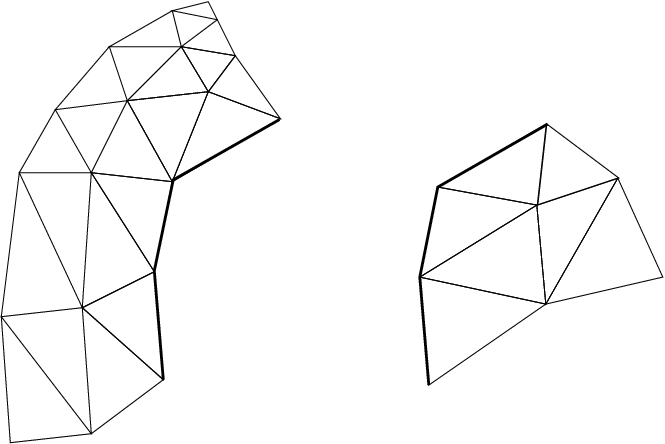
\includegraphics[width=1.5in]{fig/ghost_pre}
\end{center}
\caption{A small mesh partitioned into two pieces.}
\label{fig:ghostpre}

% \end{figure} \begin{figure} % Make sure these two figures don't get separated

\begin{center}
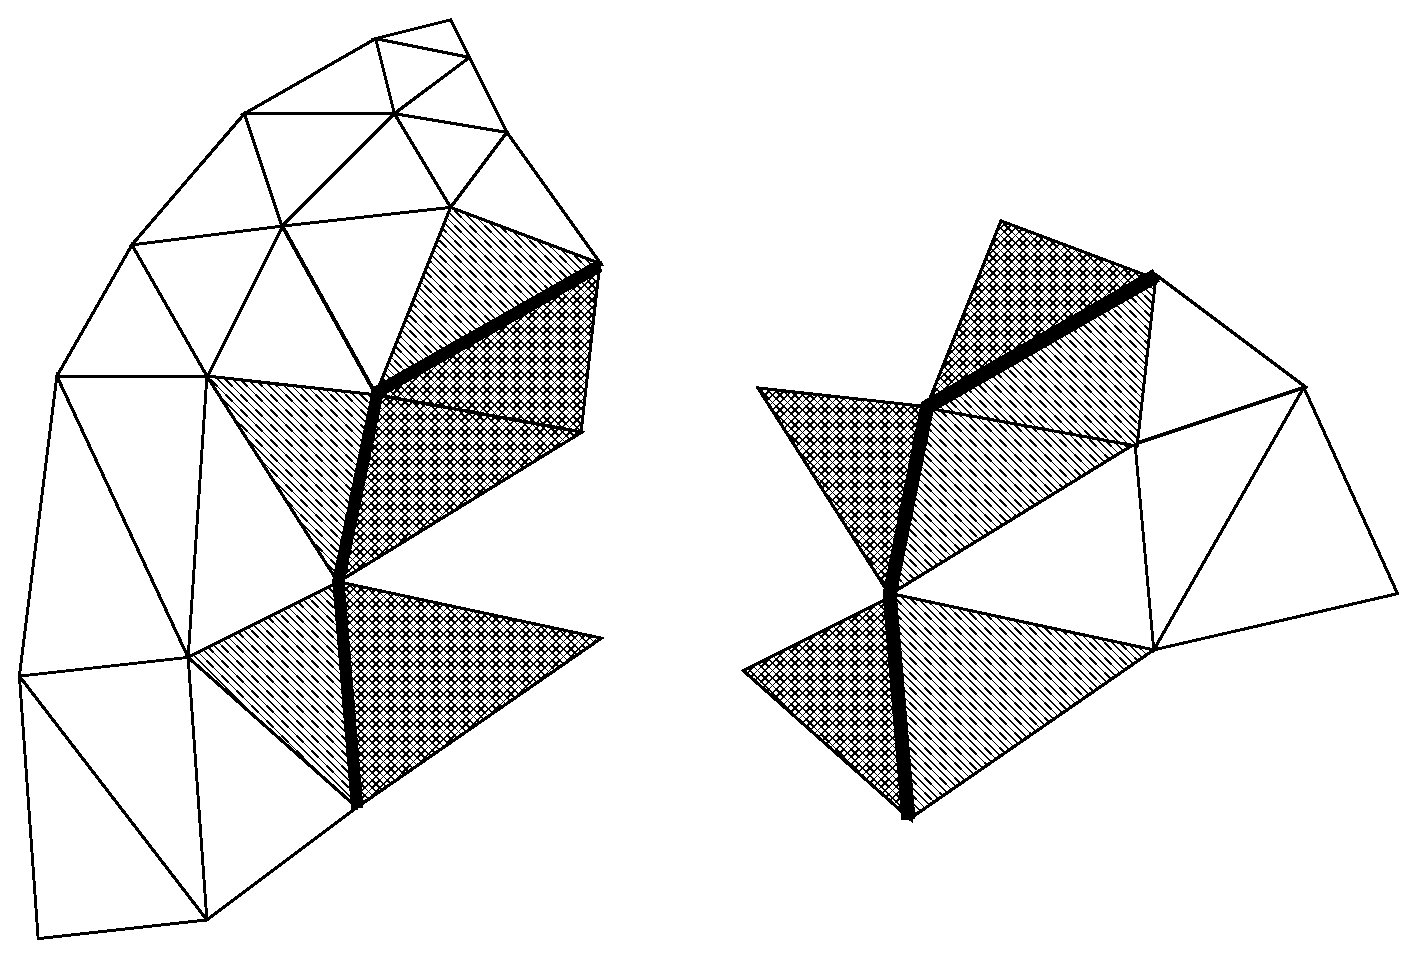
\includegraphics[width=1.5in]{fig/ghost_edge}
\end{center}
\caption{The same mesh with one layer of edge-adjacent ghosts.}
\label{fig:ghostedge}

% \end{figure} \begin{figure}

\begin{center}
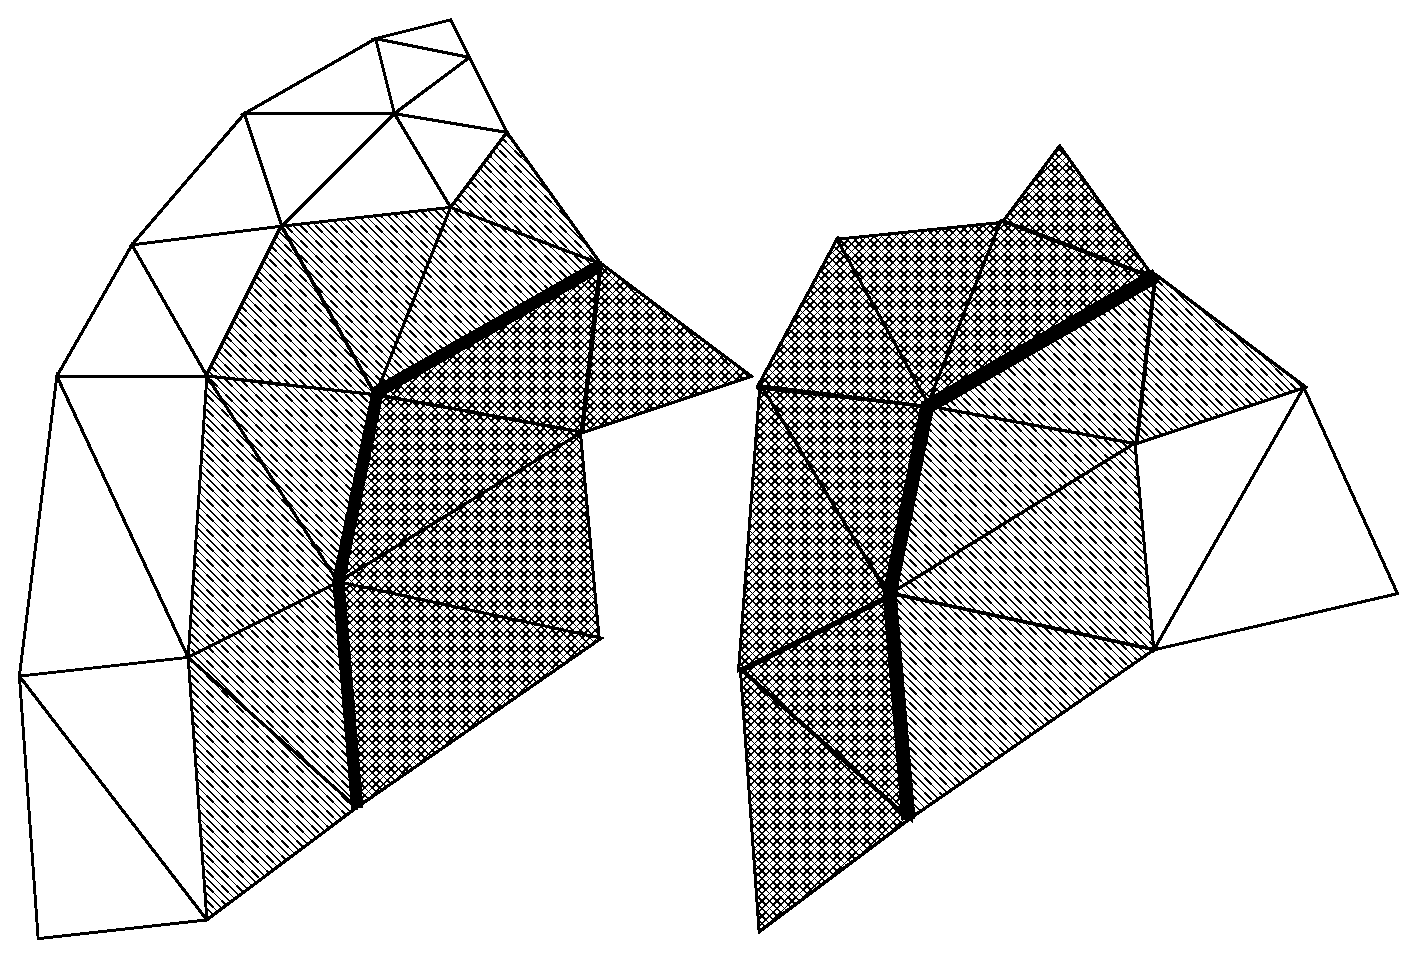
\includegraphics[width=1.5in]{fig/ghost_node}
\end{center}
\caption{The same mesh with one layer of node-adjacent ghosts.}
\label{fig:ghostnode}
\end{figure}


In Figure~\ref{fig:ghostpre}, we begin with a small mesh partitioned
into pieces on the left and right.  In Figure~\ref{fig:ghostedge},
we have added ghost elements (dark hashing) that share an edge with
adjacent real elements (light hatching).  In Figure~\ref{fig:ghostnode},
we add ghost elements that share at least one node with adjacent 
real elements.



\subsection{Ghost Numbering}
\label{sec:ghostnum}
Ghosts and real entities are stored by the framework
in separate lists---to access the ghost entity type, add \kw{FEM\_GHOST}
to the real entity's type.  For example, \kw{FEM\_GHOST}+\kw{FEM\_ELEM}+1 
lists the ghost elements for \uw{elType} 1.  To get the number 
of ghost nodes, you would call 
\kw{FEM\_Mesh\_get\_length}(\uw{mesh},\kw{FEM\_GHOST}+\kw{FEM\_NODE}).

\begin{figure}[h]
\begin{center}
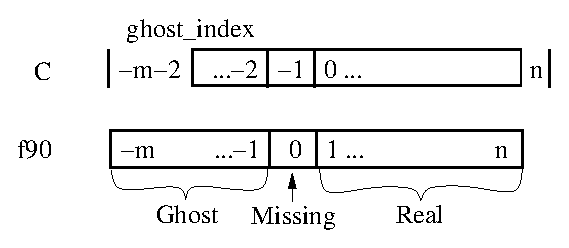
\includegraphics[width=4in]{fig/conn_indexing}
\end{center}
\caption{Node indices used in the element connectivity array.
There are $n$ real nodes and $m$ ghosts.}
\label{fig:connindexing}
\end{figure}

For real elements, the element connectivity always consists of real nodes.
But for ghost elements, the adjacent nodes may be missing, or may themselves
be ghosts.
Thus ghost element connectivity lists may include the invalid 
value -1 (in C) or 0 (in Fortran) to indicate that the corresponding 
node is not present; or may include values
less than this, which indicate the corresponding node is a ghost.
In C, ghost node $i$ is indicated by the value $-2-i$, while
in Fortran, ghost node $i$ is indicated by the value $-i$.  
This node indexing system is illustrated in Figure~\ref{fig:connindexing}, 
This indexing system is bizarre, but it allows us to keep
the real and ghost nodes clearly separate, while still
allowing real and ghost nodes to be added in increasing order
at both ends.

Since the C tests are complicated, in C we recommend using these macros:

\begin{itemize}
\item \kw{FEM\_Is\_ghost\_index}(i) returns true if $i$ represents a ghost node.
In Fortran, use the test $i$ .lt. $0$

\item \kw{FEM\_From\_ghost\_index}(i) returns the ghost node's index given its connectivity entry.
In Fortran, use the expression $-i$.

\item \kw{FEM\_To\_ghost\_index}(i) returns the connectivity entry for a given ghost node index.
In Fortran, again use the expression $-i$.
\end{itemize}

For example, a quadrilateral ghost element that is adjacent to, respectively, two real 
nodes 23 and 17, the tenth local ghost node, and one not-present node might have a 
connectivity entry of {23,17,-11,-1} (in C) or {23,17,-10,0} (in Fortran).

Applications may wish to use some other numbering,
such as by storing all the ghost nodes after all the real nodes.
The code to extract and renumber the connectivity of some 3-node triangles 
stored in FEM\_ELEM+2 would be:

\begin{alltt}
/* C version */
  int nReal=FEM\_Mesh\_get\_length(mesh,FEM\_ELEM+2);
  int nGhost=FEM\_Mesh\_get\_length(mesh,FEM\_GHOST+FEM\_ELEM+2);
  typedef int intTriplet[3];
  intTriplet *conn=new intTriplet[nReal+nGhost];
  /* Extract real triangles into conn[0..nReal-1] */
  FEM\_Mesh\_data(mesh,FEM\_ELEM+2,FEM\_CONN, &conn[0][0], 0,nReal, 3,FEM\_INDEX\_0);
  /* Extract ghost triangles into conn[nReal..nReal+nGhost-1] */
  FEM\_Mesh\_data(mesh,FEM\_GHOST+FEM\_ELEM+2,FEM\_CONN, &conn[nReal][0], 0,nGhost, 3,FEM\_INDEX\_0);
  
  /* Renumber the ghost triangle connectivity */
  for (int t=nReal;t<nReal+nGhost;t++)
    for (int i=0;i<3;i++) \{
      int in=conn[t][i]; /* uses FEM ghost node numbering */
      int out; /* uses application's ghost numbering */
      if (in==-1) \{ 
        out=some\_value\_for\_missing\_nodes; 
      \} else if (FEM\_Is\_ghost\_index(in)) \{
        out=first\_application\_ghost+FEM\_From\_ghost\_index(in);
      \} else /*regular real node*/ \{
        out=in;
      \}
      conn[t][i]=out;
    \}

! F90 version
  INTEGER, ALLOCATABLE :: conn(3,:)
  INTEGER :: nReal,nGhost,t,i,in,out
  nReal=FEM\_Mesh\_get\_length(mesh,FEM\_ELEM+2)
  nGhost=FEM\_Mesh\_get\_length(mesh,FEM\_GHOST+FEM\_ELEM+2)
  ALLOCATE(conn(3,nReal+nGhost))
  ! Extract real triangles into conn[1..nReal] 
  CALL FEM\_Mesh\_data(mesh,FEM\_ELEM+2,FEM\_CONN, conn, 1,nReal, 3,FEM\_INDEX\_1)
  ! Extract ghost triangles into conn[nReal+1..nReal+nGhost] 
  CALL FEM\_Mesh\_data(mesh,FEM\_GHOST+FEM\_ELEM+2,FEM\_CONN, conn(1,nReal+1), 1,nGhost, 3,FEM\_INDEX\_1)
  
  ! Renumber the ghost triangle connectivity 
  DO t=nReal+1,nReal+nGhost
    DO i=1,3
      in=conn(i,t) 
      IF (in .EQ. 0) out=some\_value\_for\_missing\_nodes
      IF (in .LT. 0) out=first\_application\_ghost-1+(-in)
      IF (in .GT. 0) out=in
      conn(i,t)=out
    END DO
  END DO
  
  
\end{alltt}



\subsection{Setting up the ghost layer}
The framework's ghost handling is element-centric. You specify which kinds of elements should be ghosts and how they connect by listing their faces before partitioning.  

\begin{itemize}
\item

\prototype{FEM\_Add\_ghost\_layer}
\function{void FEM\_Add\_ghost\_layer(int nodesPerFace,int doAddNodes);}
\function{SUBROUTINE FEM\_Add\_ghost\_layer(nodesPerFace,doAddNodes)}
  \args{INTEGER, INTENT(IN) :: nodesPerFace,doAddNodes}
This routine creates a new layer of ghosts around each FEM chunk. \kw{nodesPerFace} is the number of shared nodes that together form a ``face''. \kw{doAddNodes} specifies that you want ghost nodes around your ghost elements.  If \kw{doAddNodes} is 0, ghost elements will have invalid -1 (in C) or 0 (in Fortran) connectivity entries where there is no corresponding local node.

A face is an unordered ``tuple'' of nodes, and is an abstract way to describe which ghosts
your application needs---an element will be added to your chunk if it connects to at 
least one of your elements' faces.  For example, if you have a 3D, tetrahedral element that require ghosts 
on all 4 of its sides, this is equivalent to requiring ghosts of every element that shares all 3
nodes of one of your triangular faces, so for you a face is a 3-node triangle.  If you have a 2D shape
and want edge-adjacency, for you a face is a 2-node edge.  If you want node-adjacent ghosts,
a face is a single node.

Calling this routine several times creates several layers of ghost elements, and the different layers need not have the same parameters.

\item
\prototype{FEM\_Add\_ghost\_elem}
\function{void FEM\_Add\_ghost\_elem(int elType,int facesPerElem,const int *elem2face);}
\function{SUBROUTINE FEM\_Add\_ghost\_elem(elType,facesPerElem,elem2face)}
  \args{INTEGER, INTENT(IN) :: elType,facesPerElem}
  \args{INTEGER, INTENT(IN) :: elem2face(nodesPerFace,facesPerElem)}

This call is used to specify which type of element is to be added to the current ghost layer. \kw{facesPerElem} and \kw{elem2face} specify a mapping between each element and the surrounding faces.  The \kw{elem2face} table lists, for each face, the nodes of this element which form the face, specified as element-local numbers---indices into this element's connectivity entry. The \kw{elem2face} table should have nodesPerFace*facesPerElem entries, and no entry should be greater than nodePerEl for that element type.

Because all faces must take up the same space in the array,
\kw{elem2face} can include special indices--- -1 for C, 0 for Fortran---that indicate the
corresponding face is actually shorter than usual.  For example, if \kw{nodesPerFace} for this layer
is 4, for 4-node quadrilateral faces, you could set one entry in \kw{elem2face} to -1 to specify
this is a 3-node triangular face.  Faces of different lengths will never match, so this is just
a simple way to add ghosts from two kinds of faces at once.

\end{itemize}

The above two routines are always used together. For example, if your elements are 3-node triangles and you only require one shared node for inclusion in a single ghost layer, you would use:
\begin{alltt}
   FEM\_Add\_ghost\_layer(1,1); /* 1 node per face: node adjacency */
   const static int tri2node[]=\{0,1,2\};
   FEM\_Add\_ghost\_elem(0,3,tri2node); /* triangles are surrounded by 3 nodes */
\end{alltt}

If you require two shared nodes (a shared edge), the code will look like:
\begin{alltt}    
   FEM\_Add\_ghost\_layer(2,1); /* 2 nodes per face: edge adjacency */
   const static int tri2edge[]=\{0,1,  1,2,  2,0\};
   FEM\_Add\_ghost\_elem(0,3,tri2edge); /*triangles are surrounded by 3 edges */
\end{alltt}


\subsection{Symmetries and Ghosts--Geometric Layer}

The FEM framework can create ghosts not only of things that are on other 
processors, but also for various problem symmetries, like mirror reflection,
and various types of periodicities.  The interface for these ghosts is 
simple---you ask for the symmetries to be created, then you will get 
extra ghosts along each symmetry boundary.  The symmetry ghosts are
updated properly during any communication, even if the symmetry ghosts
are ghosts of real local elements from the same chunk.


\begin{figure}[h]
\begin{center}
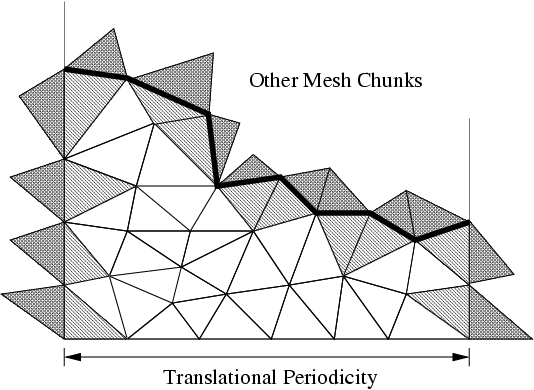
\includegraphics[width=3in]{fig/sym_ghost}
\end{center}
\caption{Illustrating symmetry ghost elements.}
\label{fig:symghost}
\end{figure}

Figure~\ref{fig:symghost} shows a chunk of a mesh for a 
rectangular domain with horizontal linear translational periodicity---that 
is, the domain repeats horizontally.
Symmetry ghosts lie along the left and right sides; ordinary cross-processor
parallel ghosts lie along the top edge where this chunk joins up with the
rest of the domain; and the external boundary along the bottom of the chunk
has no ghosts.



\prototype{FEM\_Add\_linear\_periodicity}
\function{void FEM\_Add\_linear\_periodicity(
        int nFaces,int nPer,
        const int *facesA,const int *facesB,
        int nNodes,const double *nodeLocs
        );}
\function{
SUBROUTINE FEM\_Add\_linear\_periodicity(nFaces,nPer,facesA,facesB,
                                nNodes,nodeLocs)}
  \args{INTEGER, INTENT(IN) :: nFaces, nPer, nNodes}
  \args{INTEGER, INTENT(IN) :: facesA(nPer,nFaces), facesB(nPer,nFaces)}
  \args{double precision, INTENT(IN) :: nodeLocs(3,nNodes)}

Make facesA and facesB match up under linear translation.
Each face of facesA must match up with exactly one face of
facesB, but both the faces and the nodes within a face can be
permuted in any order---the order is recovered by matching 3d locations
in the nodeLocs array.

This call can be repeated, for example if the domain is periodic along several
directions.  This call can only be issued from \kw{init()}.



\prototype{FEM\_Sym\_coordinates}
\function{void FEM\_Sym\_coordinates(int elTypeOrMinusOne,double *locs);}
\function{SUBROUTINE FEM\_Sym\_coordinates(elTypeOrZero,locs)}
  \args{INTEGER, INTENT(IN) :: elTypeOrZero}
  \args{double precision, intent(inout) :: locs(3,<number of items>)}

This call adjusts the 3d locations listed in \kw{locs} so they respect the symmetries
of their corresponding item.  If elTypeOrZero is an element type,
the locations are adjusted to match with the corresponding element;
if elTypeOrZero is zero, the locations are adjusted to match up with
the corresponding node.

This call is needed because symmetry ghost nodes and elements
initially have their original locations, which must be adjusted
to respect the symmetry boundaries.  Thus this call is needed
both for initial location data (e.g., from \kw{FEM\_Get\_node\_data})
as well as any communicated location data (e.g., from
\kw{FEM\_Update\_ghost\_field}).

This call can only be issued from \kw{driver()}.



\subsection{Advanced Symmetries and Ghosts--Lower Layer}

The geometric symmetry layer in the preceeding section is actually
a thin wrapper around this lower, more difficult to use layer.

\prototype{FEM\_Set\_sym\_nodes}
\function{void FEM\_Set\_sym\_nodes(const int *canon,const int *sym);}
\function{SUBROUTINE FEM\_Set\_sym\_nodes(canon,sym)}
  \args{INTEGER, INTENT(IN) :: canon(nNodes)}
  \args{INTEGER, INTENT(IN) :: sym(nNodes)}

This call describes all possible symmetries in an extremely terse format.
It can only be called from \kw{init()}.
The ``canonicalization array'' canon maps nodes to their canonical 
representative---if canon($i$)=canon($j$), nodes $i$ and $j$ are 
images of each other under some symmetry.  The sym array has bits set
for each symmetry boundary passing through a node.

For example, a 2d domain with 6 elements A, B, C, D, E, and F and 12 
nodes numbered 1-12 that is 
mirror-symmetric on the horizontal boundaries but periodic in the 
vertical boundaries would look like:

\begin{alltt}
   D^'|  D^ |  E^ |  F^ |  F^`
   -  1  -  2  -  3  -  4  -
   A' |  A  |  B  |  C  |  C`
   -  5  -  6  -  7  -  8  -
   D' |  D  |  E  |  F  |  F`
   -  9  - 10  -  11 -  12 -
   Av'|  Av |  Bv |  Cv |  Cv`

  v indicates the value has been shifted down (bottom boundary),
  ^ indicates the value has been shifted up (top boundary),
  ' indicates the value has been copied from the left (right boundary),
  ` indicates the value has been copied from the right (left boundary).
\end{alltt}

If we mark the left border with 1, the top with 2, the right with 4,
and the bottom with 8, this situation is indicated by topologically pasting the 
top row to the bottom row by setting their \kw{canon} entries equal, and 
marking each node with its symmetries.

\begin{center}
\begin{tabular}{|l|l|l|}\hline
  Node & \kw{canon} &  \kw{sym}              \\\hline
    1  &    1  &      3 (left + top)   \\
    2  &    2  &      2 (top)   \\
    3  &    3  &      2 (top)   \\
    4  &    4  &      6 (top + right)   \\
    5  &    5  &      1 (left)   \\
    6  &    6  &      0 (none)   \\
    7  &    7  &      0 (none)   \\
    8  &    8  &      4 (right)   \\
    9  &    1  &      9 (left+bottom)    \\
    10 &    2  &      8 (bottom)   \\
    11 &    3  &      8 (bottom)   \\
    12 &    4  &      12 (bottom+right)   \\
\hline
\end{tabular}
\end{center}


\prototype{FEM\_Get\_sym}
\function{void FEM\_Get\_sym(int elTypeOrMinusOne,int *destSym);}
\function{void FEM\_Get\_sym(elTypeOrZero,destSym);}
  \args{INTEGER, INTENT(IN) :: elTypeOrMinusOne }
  \args{INTEGER, INTENT(OUT) :: destSym(nItems)}

This call extracts the list of symmetry conditions that apply to 
an item type.  If elType is an element type, it returns the
symmetry conditions that apply to that element type; if elType is
-1 (zero for Fortran), it returns the symmetry conditions that apply
to the nodes.  Symmetry conditions are normally only nonzero
for ghost nodes and elements.


Mirror symmetry conditions are not yet supported, nor are
multiple layers of symmetry ghosts, but both should be easy to add
without changing this interface.

% FIXME: document these
% void FEM\_Set\_partition(int *elem2chunk)
% int FTN\_NAME(FEM\_GET\_COMM\_PARTNERS,fem\_get\_comm\_partners)(void)
% int FTN\_NAME(FEM\_GET\_COMM\_PARTNER,fem\_get\_comm\_partner)(int *partnerNo)
% int FTN\_NAME(FEM\_GET\_COMM\_COUNT,fem\_get\_comm\_count)(int *partnerNo)
% void FTN\_NAME(FEM\_GET\_COMM\_NODES,fem\_get\_comm\_nodes)(int *pNo,int *nodeNos)
% void FTN\_NAME(FEM\_GET\_ELEM\_NUMBERS,fem\_get\_elem\_numbers)(int *gNo)
% void fem\_get\_node\_numbers(int *gNo)





%%%%%%%%%%%%%%%%%%%%%% Old Mesh %%%%%%%%%%%%%%%%%%%%%%%%%%

\section{Older Mesh Routines}
These routines have a simpler, but less flexible interface
than the general routines described in Section~\ref{sec:entities}.  Because they are 
easy to implement in terms of the new routines, they will remain
part of the framework indefinitely.
These routines always use the default mesh, as returned by 
\kw{FEM\_Mesh\_default\_read} and \kw{FEM\_Mesh\_default\_write}.


\prototype{FEM\_Get/Set\_elem}
\function{void FEM\_Set\_elem(int elType,int  nEl,int  doublePerEl,int  nodePerEl);}
\function{void FEM\_Get\_elem(int elType,int *nEl,int *doublePerEl,int *nodePerEl);}
\function{SUBROUTINE FEM\_Set\_elem(elType,nEl,doublePerEl,nodePerEl)}
  \args{INTEGER, INTENT(IN)  :: elType,nEl,doublePerEl,nodePerEl}
\function{SUBROUTINE FEM\_Get\_elem(elType,nEl,doublePerEl,nodePerEl)}
  \args{INTEGER, INTENT(IN)  :: elType}
  \args{INTEGER, INTENT(OUT) :: nEl,doublePerEl,nodePerEl}

     Describe/retreive the number and type of elements.  \kw{ElType} is a
user-defined small, unique element type tag.  \kw{nEl} is the number of elements 
being registered.  \kw{doublesPerEl} and \kw{nodePerEl} are the number of doubles of user data, and nodes (respectively) associated with each element.

     \kw{doublePerEl} or \kw{nodePerEl} may be zero, indicating that no user
data or connectivity data (respectively) is associated with the element.

     You can make this and any other mesh setup calls in any order---there is no need 
to make them in linearly increasing order.  However, for a given type of element
\kw{FEM\_Set\_elem} must be called before setting that element's connectivity or data.


\prototype{FEM\_Get/Set\_elem\_conn}
\function{void FEM\_Set\_elem\_conn(int elType,const int *conn);}
\function{void FEM\_Get\_elem\_conn(int elType,int *conn);}
\function{SUBROUTINE FEM\_Set\_elem\_conn\_r(elType,conn)}
  \args{INTEGER, INTENT(IN)  :: elType}
  \args{INTEGER, INTENT(IN),  dimension(nodePerEl,nEl) :: conn}
\function{SUBROUTINE FEM\_Get\_elem\_conn\_r(elType,conn)}
  \args{INTEGER, INTENT(IN)  :: elType}
  \args{INTEGER, INTENT(OUT), dimension(nodePerEl,nEl) :: conn}
\function{SUBROUTINE FEM\_Set\_elem\_conn\_c(elType,conn)}
  \args{INTEGER, INTENT(IN)  :: elType}
  \args{INTEGER, INTENT(IN),  dimension(nEl,nodePerEl) :: conn}
\function{SUBROUTINE FEM\_Get\_elem\_conn\_c(elType,conn)}
  \args{INTEGER, INTENT(IN)  :: elType}
  \args{INTEGER, INTENT(OUT), dimension(nEl,nodePerEl) :: conn}

     Describe/retreive the element connectivity array for this element
     type.  The connectivity array is indexed by the element number,
     and gives the indices of the nodes surrounding the element.  It is
     hence \kw{nodePerEl*nEl} integers long.

     The C version array indices are zero-based, and must be stored in
     row-major order (a given element's surrounding nodes are stored
     contiguously in the conn array).  The Fortran version indices are
     one-based, and are available in row-major (named \_r) and
     column-major (named \_c) versions.  We recommend row-major storage
     because it results in better cache utilization (because the nodes
     around an element are stored contiguously).
     
     In this older interface, ghost nodes are indicated by invalid, 

\prototype{FEM\_Get/Set\_node}
\function{void FEM\_Set\_node(int  nNode,int  doublePerNode);}
\function{void FEM\_Get\_node(int *nNode,int *doublePerNode);}
\function{SUBROUTINE FEM\_Set\_node(nNode,doublePerNode)}
  \args{INTEGER, INTENT(IN)  :: nNode,doublePerNode}
\function{SUBROUTINE FEM\_Get\_node(nNode,doublePerNode)}
  \args{INTEGER, INTENT(OUT) :: nNode,doublePerNode}

     Describe/retreive the number of nodes and doubles of user data
     associated with each node.  There is only one type of node, so no
     \kw{nodeType} identifier is needed.

     \kw{doublePerNode} may be zero, indicating that no user data is
     associated with each node.
     

\subsection{Old Mesh Data}
\prototype{FEM\_Get/Set\_data}
\function{void FEM\_Set\_node\_data(const double *data);}
\function{void FEM\_Get\_node\_data(double *data);}
\function{void FEM\_Set\_elem\_data(int elType,const double *data);}
\function{void FEM\_Get\_elem\_data(int elType,double *data);}
\function{SUBROUTINE FEM\_Set\_node\_data\_r(data)}
  \args{REAL*8, INTENT(IN),  dimension(doublePerNode,nNode)  :: data}
\function{SUBROUTINE FEM\_Get\_node\_data\_r(data)}
  \args{REAL*8, INTENT(OUT), dimension(doublePerNode,nNode)  :: data}
\function{SUBROUTINE FEM\_Set\_node\_data\_c(data)}
  \args{REAL*8, INTENT(IN),  dimension(nNode,doublePerNode)  :: data}
\function{SUBROUTINE FEM\_Get\_node\_data\_c(data)}
  \args{REAL*8, INTENT(OUT), dimension(nNode,doublePerNode)  :: data}

\function{SUBROUTINE FEM\_Set\_elem\_data\_r(elType,data)}
  \args{INTEGER, INTENT(IN)  :: elType}
  \args{REAL*8, INTENT(IN),  dimension(doublePerElem,nElem)  :: data}
\function{SUBROUTINE FEM\_Get\_elem\_data\_r(elType,data)}
  \args{INTEGER, INTENT(IN)  :: elType}
  \args{REAL*8, INTENT(OUT), dimension(doublePerElem,nElem)  :: data}
\function{SUBROUTINE FEM\_Set\_elem\_data\_c(elType,data)}
  \args{INTEGER, INTENT(IN)  :: elType}
  \args{REAL*8, INTENT(IN),  dimension(nElem,doublePerElem)  :: data}
\function{SUBROUTINE FEM\_Get\_elem\_data\_c(elType,data)}
  \args{INTEGER, INTENT(IN)  :: elType}
  \args{REAL*8, INTENT(OUT), dimension(nElem,doublePerElem)  :: data}

     Describe/retrieve the optional, uninterpreted user data associated with
each node and element.  This user data is partitioned and reassembled along
with the connectivity matrix, and may include initial conditions, node locations,
material types, or any other data needed or produced by the program.   The Fortran
arrays can be row- or column- major (see \kw{FEM\_Set\_elem\_conn} for
details).  The row-major form is preferred.



\subsection{Old Ghost Numbering}



In this older version of the framework, FEM\_Get\_node and FEM\_Get\_elem return the 
\textbf{total} number of nodes and elements, including ghosts. The routines below
return the index of the first ghost node or element, where ghosts are numbered
after all the real elements.  This old ghost numbering scheme does not work
well when adding new ghosts, which is why the new ghost numbering scheme
describes in Section~\ref{sec:ghostnum} is used in the new API.


\begin{figure}[h]
\begin{center}
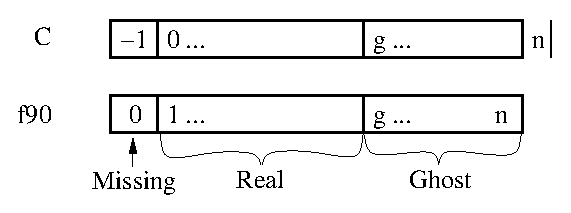
\includegraphics[width=4in]{fig/conn_indexing_old}
\end{center}
\caption{Old ghost element and node numbering.  \kw{FEM\_Get\_ghost\_*} returns $g$,
\kw{FEM\_Get\_*} returns $n$.}
\label{fig:connold}
\end{figure}



\prototype{FEM\_Get\_ghost}
\function{int FEM\_Get\_node\_ghost(void);}
\function{int FEM\_Get\_elem\_ghost(int elemType);}

The examples below iterate over the real and ghost elements using the old numbering:
\begin{alltt}
C version:
        int firstGhost,max;
        FEM\_Get\_node(\&max, \&ignored);
        firstGhost=FEM\_Get\_node\_ghost();
        for (i=0;i<firstGhost;i++)
                ... i is a real node...
        for (i=firstGhost;i<max;i++)
                ... i is a ghost node ...

Fortran version:
        call FEM\_Get\_node(max,ignored);
        firstGhost=FEM\_Get\_node\_ghost();
        do i=1,firstGhost-1
                ... i is a real node...
        end do
        do i=firstGhost,max
                ... i is a ghost node...
        end do
\end{alltt}



\subsection{Old Backward Compatability}
\prototype{FEM\_Set\_mesh}
\function{void FEM\_Set\_mesh(int nElem, int nNodes, int nodePerEl,const int* conn);}

     This is a convenience routine equivalent to:
\begin{alltt}
          FEM\_Set\_node(nNodes,0);
          FEM\_Set\_elem(0,nElem,0,nodePerEl);
          FEM\_Set\_elem\_Conn(0,conn);
\end{alltt}

\function{SUBROUTINE FEM\_Set\_mesh(nElem,nNodes,nodePerEl,conn)}
    \args{INTEGER, INTENT(IN) :: nElem, nNodes, nodePerEl}
    \args{INTEGER, INTENT(IN), dimension(nElem,nodePerEl) :: conn;}

     This is a convenience routine equivalent to:
\begin{alltt}
          CALL FEM\_Set\_node(nNodes,0)
          CALL FEM\_Set\_elem(1,nElem,0,nodePerEl)
          CALL FEM\_Set\_elem\_Conn\_c(1,conn)
\end{alltt}


\subsection{Old Sparse Data}

Sparse data is typically used to represent boundary conditions.  For
example, in a structural dynamics program typically some nodes have 
an imposed force or position.  The routines in this section are 
used to describe this kind of mesh-associated data---data that only 
applies to some ``sparse'' subset of the nodes or elements.  


\prototype{FEM\_Set\_sparse}
\function{void FEM\_Set\_sparse(int S\_id,int nRec,
         const int *nodes,int nodesPerRec,
         const void *data,int dataPerRec,int dataType);}
\function{SUBROUTINE FEM\_Set\_sparse(S\_id,nRec,nodes,nodesPerRec,data,dataPerRec,dataType)}
  \args{INTEGER, INTENT(IN) :: S\_id,nRec,nodesPerRec,dataPerRec,dataType}
  \args{INTEGER, INTENT(IN) :: nodes(nodesPerRec,nRec)}
  \args{varies,  INTENT(IN) :: data(dataPerRec,nRec)}

Register \kw{nRec} sparse data records with the framework under the number \kw{S\_id}. 
The first call to \kw{FEM\_Set\_sparse} must give a \kw{S\_id} of zero in C (1 in fortran);
and subsequent calls to \kw{FEM\_Set\_sparse} must give increasing consecutive \kw{S\_id}s.

One sparse data record consists of some number of nodes, listed in the
\kw{nodes} array, and some amount of user data, listed in the data array.
Sparse data records are copied into the chunks that contains all that record's listed 
nodes.  Sparse data records are normally used to describe mesh boundary conditions--
for node-associated boundary conditions, \kw{nodesPerRec} is 1; for triangle-associated
boundary conditions, \kw{nodesPerRec} is 3.

In general, \kw{nodePerRec} gives the number of nodes associated with each
sparse data record, and \kw{nodes} gives the actual node numbers.
\kw{dataPerRec} gives the number of data items associated with each sparse 
data record, and \kw{dataType}, one of \kw{FEM\_BYTE}, \kw{FEM\_INT},
\kw{FEM\_REAL}, or \kw{FEM\_DOUBLE}, gives the type of each data item.
As usual, you may change or delete the \kw{nodes} and \kw{data} arrays after 
this call returns.

For example, if the first set of sparse data is 17 sparse data records, each 
containing 2 nodes stored in \kw{bNodes} and 3 integers stored in \kw{bDesc}, 
we would make the call:
\begin{alltt}
/*C version*/
  FEM\_Set\_sparse(0,17, bNodes,2, bDesc,3,FEM\_INT);
! Fortran version
  CALL FEM\_Set\_sparse(1,17, bNodes,2, bDesc,3,FEM\_INT)
\end{alltt}

\prototype{FEM\_Set\_sparse\_elem}
\function{void FEM\_Set\_sparse\_elem(int S\_id,const int *rec2elem);}
\function{SUBROUTINE FEM\_Set\_sparse\_elem(S\_id,rec2elem)}
  \args{INTEGER, INTENT(IN) :: S\_id}
  \args{INTEGER, INTENT(IN) :: rec2elem(2,nRec)}

Attach the previously-set sparse records \kw{S\_id} to the given elements.
\kw{rec2elem} consists of pairs of integers---one for each sparse data record.
The first integer in the pair is the
element type to attach the sparse record to, and the second integer
gives the element number within that type.  For example, to attach
the 3 sparse records at \kw{S\_id} to the elements numbered 10, 11, and 12
of the element type \kw{elType}, use:

\begin{alltt}
/*C version*/
  int rec2elem[]={elType,10, elType,11, elType,12};
  FEM\_Set\_sparse\_elem(S\_id,rec2elem);
! Fortran version
  integer :: rec2elem(2,3);
  rec2elem(1,:)=elType
  rec2elem(2,1)=10; rec2elem(2,2)=11; rec2elem(2,3)=12;
  CALL FEM\_Set\_sparse\_elem(S\_id,rec2elem)
\end{alltt}


\prototype{FEM\_Get\_sparse}
\function{int  FEM\_Get\_sparse\_length(int S\_id);}
\function{void FEM\_Get\_sparse(int S\_id,int *nodes,void *data);}
\function{function FEM\_Get\_sparse\_length(S\_id);}
  \args{INTEGER, INTENT(IN) :: S\_id}
  \args{INTEGER, INTENT(OUT) :: FEM\_Get\_sparse\_Length}
\function{SUBROUTINE FEM\_Get\_sparse(S\_id,nodes,data);}
  \args{INTEGER, INTENT(IN) :: S\_id}
  \args{INTEGER, INTENT(OUT) :: nodes(nodesPerRec,FEM\_Get\_sparse\_Length(S\_id))}
  \args{varies,  INTENT(OUT) :: data(dataPerRec,FEM\_Get\_sparse\_Length(S\_id))}

Retrieve the previously registered sparse data from the framework.
\kw{FEM\_Get\_sparse\_length} returns the number of records of sparse
data registered under the given \kw{S\_id}; zero indicates no records
are available.  \kw{FEM\_Get\_sparse} returns you the actual nodes
(translated to local node numbers) and unchanged user data for
these sparse records.

In this old interface, there is no way to access sparse ghosts.



%%%%%%%%%%%%%%%%%%%%%%%%%%%%%%%%%%%%%%%%%%%%%%%%%%%%%%%%%%%%%%%%%%%%%%%%%%%%%%%%%%%%%%%%
\newpage
\section{Mesh Modification}


\prototype{FEM\_Update\_mesh}
\function{void FEM\_Update\_mesh(FEM\_Update\_mesh\_fn routine, int callMeshUpdated,int doWhat);}
\function{SUBROUTINE FEM\_Update\_mesh(routine,callMeshUpdated,doWhat)}
    \args{external, INTENT(IN) :: routine}
    \args{INTEGER, INTENT(IN) :: callMeshUpdated,doWhat}

Reassemble the mesh chunks from each partition into a single serial mesh,
and call the given \kw{routine} on the assembled mesh.
In this \kw{routine}, which runs on processor 0, the \kw{FEM\_Get} and \kw{FEM\_Set} routines
can manipulate the serial mesh.  The parameter \kw{callMeshUpdated}, which must
be non-zero, is passed down to \kw{routine} as \kw{routine(callMeshUpdated)}.

\kw{FEM\_Get} calls from
\kw{driver()} will only return the new mesh after a \kw{FEM\_Update\_mesh} call
where \kw{doWhat} is \kw{FEM\_MESH\_UPDATE}; otherwise \kw{FEM\_Get} from \kw{driver()} will still
return the old mesh.
\kw{FEM\_Update\_mesh} can only be called from driver; and must be called by the driver routine for
every chunk. 

%     If \kw{doRepartition} is 0, the mesh is not repartitioned, and \kw{FEM\_Update\_mesh}
%returns immediately.  If \kw{doRepartition} is 1, \kw{FEM\_Update\_mesh} blocks
%until the reassembled serial mesh is repartitioned back into chunks and redistributed.
%If \kw{doRepartition} is 2, 

\begin{center}
\begin{tabular}{|l|l|l|l|}\hline
\kw{doWhat} & Numeric & Repartition? & \kw{FEM\_Update\_mesh} \\\hline
\kw{FEM\_MESH\_OUTPUT} & 0 & No & \kw{driver()} continues alongside \kw{routine} \\
\kw{FEM\_MESH\_FINALIZE} & 2 & No & \kw{driver()} blocks until \kw{routine} finishes\\
\kw{FEM\_MESH\_UPDATE} & 1 & Yes & \kw{driver()} blocks for the new partition \\
\hline
\end{tabular}
\end{center}

For example, \kw{FEM\_Update\_mesh}(\uw{my\_output\_routine}, \uw{k}, \kw{FEM\_MESH\_OUTPUT}) 
reassembles the mesh and calls a routine named
\uw{my\_output\_routine(k)} while the driver routines continue with the computation.
This might be useful, for example, for writing out intermediate solutions as a 
single file; writing outputs from \kw{driver()} is more efficient but often results 
in a separate file for each mesh chunk.

   To block the driver routines during a call to a routine named
\uw{my\_finalize\_routine(k)}, such as 
at the end of the computation when the drivers have no other work to do, 
use \kw{FEM\_Update\_mesh}(\uw{my\_finalize\_routine}, \uw{k}, \kw{FEM\_MESH\_FINALIZE}).

     To reassemble, modify, and repartition the mesh, use
\kw{FEM\_Update\_mesh}(\uw{my\_update\_routine}, \uw{k}, \kw{FEM\_MESH\_UPDATE}).
It may be easier to perform major mesh modifications from \uw{my\_update\_routine(k)} than
the drivers, since the entire serial mesh is available to \uw{my\_update\_routine(k)}.

     \kw{FEM\_Update\_mesh} reassembles the serial mesh with an attempt to
     preserve the element and node global numbering.  If the new mesh
     has the same number and type of elements and nodes, the global
     numbers (and hence serial mesh) will be unchanged.  If new
     elements or nodes are added at each chunk, they will be assigned
     new unique global numbers.  If elements or nodes are removed,
     their global numbers are not re-used-- you can detect the
     resulting holes in the serial mesh since the user data associated
     with the deleted elements will be all zero.  Generally, however, it
     is less error-prone to perform mesh modifications only in \kw{driver()}
     or only in an update routine, rather than some in both.




\section{IDXL Communication}

The FEM framework's communication layer is called IDXL. This small library handles sending and receiving data to and from a sparse subset of 1D indices into a user array.  The sparse index subset is called an "Index List", hence the name of the library.


\subsection{Index Lists}
\label{sec:IDXL}
An Index List is the fundamental data structure of the IDXL library---for example, the list of shared nodes is an Index List.  IDXL includes routines for building, combining, and sending and receiving Index Lists.

An Index List, as you might expect, is a list of indices that need to be sent and received.  An Index List includes both the indices that need to be sent, as well as the indices to be received, from each chunk.

Consider two chunks $a$ and $b$ where $b$ needs some information $a$ has, such as if $b$ has ghosts of real elements on $a$.  $a$'s Index List thus has a send portion with the $a$-local indices for the elements $a$ sends; and $b$'s Index List contains a receive portion with the $b$-local indices for the elements $b$ receives.  Thus across processors, the corresponding send and receive portions of $a$ and $b$'s Index Lists match, as shown in Figure~\ref{fig:indexlists}.


\begin{figure}[h]
\begin{center}
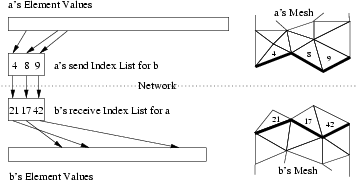
\includegraphics[width=5in]{fig/indexlists}
\end{center}
\caption{Illustrating how Index Lists match up $a$'s source elements with $b$'s ghost elements.}
\label{fig:indexlists}
\end{figure}



%%%%%%%%%%%%%%%%%%% Index Lists %%%%%%%%%%%%%%%%%%%%
\subsubsection{Index List Calls}

You refer to an Index List via an opaque handle---in C, the integer typedef \kw{IDXL\_t}; in Fortran, a bare INTEGER.  


\prototype{FEM\_Comm\_shared}
\function{IDXL\_t FEM\_Comm\_shared(int mesh,int entity);}
\function{INTEGER function FEM\_Comm\_shared(mesh,entity)}
  \args{INTEGER, INTENT(IN)  :: mesh,entity}

Return a read-only copy of the Index List of shared nodes.  The send and receive portions of this list are identical, because each shared node is both sent and received.  Shared nodes are most often used with the \kw{send/sum} communication pattern.

Must be called from driver.  \kw{mesh} must be a reading mesh. \kw{entity} must be \kw{FEM\_NODE}.  You may not call \kw{IDXL\_Destroy} on the returned list.


\prototype{FEM\_Comm\_ghost}
\function{IDXL\_t FEM\_Comm\_ghost(int mesh,int entity);}
\function{INTEGER function FEM\_Comm\_ghost(mesh,entity)}
  \args{INTEGER, INTENT(IN)  :: mesh,entity}

Return a read-only copy of the Index List of ghost entities.  The send portion of this list contains real, interior entities, which are sent away; the receive portion of the list contains the ghost entites, which are received. Ghosts are most often used with the \kw{send/recv} communication pattern.

Elements to be sent out are listed starting at zero (one in Fortran); but ghost elements to be received are also listed starting at zero (one in Fortran).  If real and ghost elements are kept in separate arrays, this is usable as-is; but if ghosts and real elements are kept together, you will need to shift the ghost indices using \kw{IDXL\_Combine} or \kw{IDXL\_Shift}. 

This routine must be called from driver.  \kw{mesh} must be a reading mesh. \kw{entity} must not include \kw{FEM\_GHOST}--ghosts are already included.  You may not call \kw{IDXL\_Destroy} on the returned list.


\prototype{IDXL\_Create}
\function{IDXL\_t IDXL\_Create(void);}
\function{INTEGER function IDXL\_Create()}

Create a new, empty Index List. This list can then be filled up using \kw{IDXL\_Copy} or \kw{IDXL\_Combine}.

Must be called from driver.  You must eventually call \kw{IDXL\_Destroy} on the returned list.


\prototype{IDXL\_Combine}
\function{void IDXL\_Combine(IDXL\_t dest,IDXL\_t src,int startSend,int startRecv);}
\function{SUBROUTINE IDXL\_Combine(dest,src,startSend,startRecv)}
  \args{INTEGER, INTENT(IN)  :: dest,src,startSend,startRecv}

Add the shifted contents of the src Index List to dest.  The send portion of src is shifted so the first index sent will be startSend; for a ghost index list this is the index of the first sent real entity. The receive portion of src is similarly shifted so the first index received will be startRecv; for a ghost index list this is the index of the first received ghost entity.  

This routine does not check for duplicates---if an index originally appears in dest and the also in the shifted src, it will be listed twice.


\subsubsection{Advanced Index List Calls}

\prototype{IDXL\_Destroy}
\function{void IDXL\_Destroy(IDXL\_t l);}
\function{SUBROUTINE IDXL\_Destroy(l)}
  \args{INTEGER, INTENT(IN)  :: l}

Destroy this Index List, and free the list storage allocated by the framework.  Only call this routine with lists you created using \kw{IDXL\_Create}; not lists obtained directly from the FEM framework.

\prototype{IDXL\_Print}
\function{void IDXL\_Print(IDXL\_t l);}
\function{SUBROUTINE IDXL\_Print(l)}
  \args{INTEGER, INTENT(IN)  :: l}

Print out the contents of this Index List.  This routine shows both the send and receive indices on the list, for each chunk we communicate with.


\prototype{IDXL\_Copy}
\function{void IDXL\_Copy(IDXL\_t dest,IDXL\_t src);}
\function{SUBROUTINE IDXL\_Print(dest,src)}
  \args{INTEGER, INTENT(IN)  :: dest,src}

Copy the contents of the source Index List into the destination Index List, which should be empty.

\prototype{IDXL\_Shift}
\function{void IDXL\_Shift(IDXL\_t l,int startSend,int startRecv);}
\function{SUBROUTINE IDXL\_Shift(l,startSend,startRecv)}
  \args{INTEGER, INTENT(IN)  :: l,startSend,startRecv}

Like \kw{IDXL\_Combine}, but only shifts the indices within a single list.


\prototype{IDXL\_Add\_entity}
\function{void IDXL\_Add\_entity(int newIdx,int nBetween,int *between);}
\function{SUBROUTINE IDXL\_Add\_node(newIdx,nBetween,between)}
    \args{INTEGER, INTENT(IN) :: newIdx,nBetween}
    \args{INTEGER, INTENT(IN) :: between(nBetween)}

This call adds a new entity, with local index \kw{newIdx}, to this Index List.  The new entity is sent or received by each chunk that sends or receives all the entites listed in the between array.  For example, when adding a new node along an edge, nBetween is 2 and between lists the endpoints of the edge; this way if the edge is shared with some chunk, the new node will be shared with that chunk.

This routine only affects the current chunk-- no other chunks are affected.  To ensure the communication lists match, \kw{IDXL\_Add\_entity} must be called on all the chunks that send or receive the entity, to create the local copies of the entity.

\kw{IDXL\_Add\_entity} adds the new entity to the end of the communication list, and so must be called in the same order on all the chunks that share the new entity.  For example, if two new nodes $x$ and $y$ are added between chunks $a$ and $b$, if chunk $a$ calls \kw{IDXL\_Add\_entity} with its local number for $x$ before it calls \kw{IDXL\_Add\_entity} with its local number for $y$, chunk $b$ must also add its copy of node $x$ before adding $y$.

% FIXME: implement, and document, IDXL\_Sort\_2d and IDXL\_Sort\_3d

%%%%%%%%%%%%%%%%%%% Layout %%%%%%%%%%%%%%%%%%%%
\subsection{Data Layout}
\label{sec:IDXLLayout}
IDXL is designed to send and receive data directly out of your arrays, with no intermediate copying.  This means IDXL needs a completely general method for specifying how you store your data in your arrays.  Since you probably don't change your storage layout at runtime, you can create a ``data layout'' once at the beginning of your program, then use it repeatedly for communication.

IDXL Layouts are normally used to describe arrays of data associated with nodes or elements.  The layout abstraction allows you to use IDXL routines to communicate any sort of data, stored in a variety of formats.

Like Index Lists, Layouts are referred to via an opaque handle---in a C program via the integer typedef IDXL\_Layout\_t, and in Fortran via a bare integer.

\subsubsection{Layout Routines}

In most programs, the data to be communicated is a dense array of data of one type.  In this case, there is only one layout routine you need to know:

\prototype{IDXL\_Layout\_create}
\function{IDXL\_Layout\_t IDXL\_Layout\_create(int type,int width);}
\function{INTEGER function IDXL\_Layout\_create(type,width)}
    \args{INTEGER, INTENT(IN) :: type,width}

The simplest data layout to describe---a dense array of this IDXL datatype, indexed by entity number, with \kw{width} pieces of data per entity. Note that the number of entities is not stored with the layout--the number of entities to be communicated depends on the communication routine.

The IDXL datatypes are:
\begin{center}
\begin{tabular}{|l|l|l|}\hline
IDXL Datatype & C Datatypes & Fortran Datatypes \\\hline
\kw{IDXL\_BYTE} & unsigned char & INTEGER*1 \\
               & char & LOGICAL*1 \\
\kw{IDXL\_INT} & int & INTEGER \\
\kw{IDXL\_REAL} & float & SINGLE PRECISION \\
                &  & REAL*4 \\
\kw{IDXL\_DOUBLE} & double & DOUBLE PRECISION \\
                  &  & REAL*8 \\
\hline
\end{tabular}
\end{center}

For example, if you keep a dense array with 3 doubles of force per node, you'd call this routine as:

\begin{alltt}
// C++ version:
     double *force=new double[3*n];
     IDXL\_Layout\_t force\_layout=IDXL\_Layout\_create(IDXL\_DOUBLE,3);

! F90 Version
     double precision, allocatable :: force(:,:)
     integer :: force\_layout
     ALLOCATE(force(3,n)) ! (could equivalently use force(3*n) )
     force\_layout=IDXL\_Layout\_create(IDXL\_DOUBLE,3)

\end{alltt}

This routine was once called \kw{FEM\_Create\_simple\_field}.


\subsubsection{Advanced Layout Routines}
\label{sec:IDXLLayoutoffset}

These advanced routines are only needed if you want to exchange data stored in an array of user-defined types.  Most programs only need \kw{IDXL\_Layout\_create}.

\prototype{IDXL\_Layout\_offset}
\function{IDXL\_Layout\_t IDXL\_Layout\_offset(int type, int width, int offsetBytes, int distanceBytes,int skewBytes);}
\function{INTEGER function IDXL\_Layout\_offset(type,width,offsetBytes,distanceBytes,skewBytes)}
    \args{INTEGER, INTENT(IN) :: type,width,offsetBytes,distanceBytes,skewBytes}

The most general data layout--an array indexed by entity, containing \kw{width} pieces of data per entity.  This routine expands on \kw{IDXL\_Layout\_create} by adding support for user-defined types or other unusual data layouts.  You describe your layout by giving various in-memory byte offsets that describe the data is stored. Again, the number of entities is not stored with the layout--the number of entities to be communicated depends on the communication routine.

\begin{itemize}
  \item \kw{offsetBytes} The number of bytes from the start of the array to the start of the data.
  \item \kw{distanceBytes} The number of bytes taken by one entity.
  \item \kw{skewBytes} The number of bytes between each piece of data.  Since this can almost always be determined from the size of the base data type, this parameter can be left as zero.
\end{itemize}

\begin{figure}[h]
\begin{center}
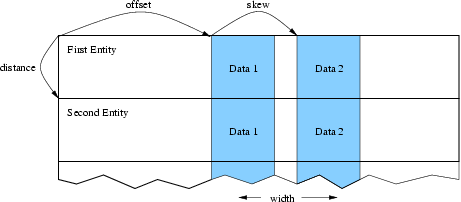
\includegraphics[width=5in]{fig/layout}
\end{center}
\caption{Describing a complex data layout.}
\label{fig:layout}
\end{figure}

For example, if your node data is all stored in a struct (in fortran, a named TYPE), offsetBytes gives the distance between the start of the struct and the force; and distanceBytes gives the size in bytes of the struct.  

In C, the offsetof and sizeof keywords are useful for finding these values.  In Fortran, we provide a special routine called \kw{foffsetof} that returns the distance, in bytes, between its two arguments.

\begin{alltt}
// C++ version:
     typedef struct \{
        double d[3], v[3], force[3], a[3];
        double m;
     \} node;
     node *nodes=new node[n];
     IDXL\_Layout\_t force\_layout=IDXL\_Layout\_offset(IDXL\_DOUBLE,3,
              offsetof(node,force),sizeof(node),0);

! F90 Version
     TYPE node 
        DOUBLE PRECISION :: d(3), v(3), force(3), a(3)
        DOUBLE PRECISION :: m
     END TYPE
     integer :: force\_layout
     ALLOCATE(nodes(n))
     force\_layout=IDXL\_Layout\_create(IDXL\_DOUBLE,3,
   &          foffsetof(nodes(1),nodes(1)\%force),
   &          foffsetof(nodes(1),nodes(2)),0)
\end{alltt}


\prototype{IDXL\_Layout\_destroy}
\function{void IDXL\_Layout\_destroy(IDXL\_Layout\_t layout);}
\function{SUBROUTINE IDXL\_Layout\_destroy(layout)}
  \args{INTEGER, INTENT(IN)  :: layout}

Destroy this Layout.  You only need call this routine if you repeatedly create layouts.

\prototype{IDXL\_Get\_layout\_type}
\function{int IDXL\_Get\_layout\_type(IDXL\_Layout\_t layout);}
\function{INTEGER function IDXL\_Get\_layout\_type(layout)}

Return the IDXL datatype for this layout.

\prototype{IDXL\_Get\_layout\_width}
\function{int IDXL\_Get\_layout\_width(IDXL\_Layout\_t layout);}
\function{INTEGER function IDXL\_Get\_layout\_width(layout)}

Return the layout width---the number of data items that are communicated
per entity.

\prototype{IDXL\_Get\_layout\_distance}
\function{int IDXL\_Get\_layout\_distance(IDXL\_Layout\_t layout);}
\function{INTEGER function IDXL\_Get\_layout\_distance(layout)}

Return the layout distance---the number of bytes between successive
entity's data items.



\subsubsection{Layout Compatability Routines}

Before IDXL was made a separate library, FEM included these routines,
which are still preserved for backward compatability.

\prototype{FEM\_Create\_simple\_field}
\function{IDXL\_Layout\_t FEM\_Create\_simple\_field(int type,int width);}
\function{INTEGER function FEM\_Create\_simple\_field(type,width)}
  \args{INTEGER, INTENT(IN)  :: type,width}

This routine is completely interchangable to \kw{IDXL\_Layout\_create}.


\prototype{FEM\_Create\_field}
\function{int FEM\_Create\_field(int type,int width,int offset,int distance);}
\function{INTEGER function FEM\_Create\_field(type, width, offset, distance)}
  \args{INTEGER, INTENT(IN)  :: type, width, offset, distance}

This routine is like a call to \kw{IDXL\_Layout\_offset} with the rarely
used \kw{skewBytes} set to zero.



%%%%%%%%%%%%%%%%%%% Communication %%%%%%%%%%%%%%%%%%%%
\subsection{IDXL Communication}
\label{sec:IDXLComm}
This section brings together all the pieces of IDXL: Index Lists are used to determine what to send and what to receive and Layouts are used to determine where to get and put the communicated data.


\subsubsection{Communication Routines}

\prototype{IDXL\_Comm\_sendsum}
\function{void IDXL\_Comm\_sendsum(IDXL\_Comm\_t comm,IDXL\_t indices,IDXL\_Layout\_t layout,void *data);}
\function{SUBROUTINE IDXL\_Comm\_sendsum(comm,indices,layout,data)}
  \args{INTEGER, INTENT(IN)  :: comm,indices,layout}
  \args{varies, INTENT(INOUT) :: data}

Sum these \kw{indices} of shared entites across all chunks that share them.
The user \kw{data} array is interpreted according to the given \kw{layout}.

If \kw{comm} is zero, this routine is blocking and finishes the communication immediately.
If \kw{comm} is not zero, this routine is non-blocking and equivalent to a call to 
\kw{IDXL\_Comm\_send} followed by a call to \kw{IDXL\_Comm\_sum}.

This routine is typically used to sum up partial values on shared nodes.
It is a more general version of the old FEM routine \kw{FEM\_Update\_field}.
For example, to sum up the shared-node values in a 3d \uw{force} vector indexed 
by node, you would use:

\begin{alltt}
// C++ version:
     double *force=new double[3*nNodes];
     IDXL\_Layout\_t force\_layout=IDXL\_Layout\_create(IDXL\_DOUBLE,3);
     IDXL\_t shared\_indices=FEM_Comm_shared(mesh,FEM_NODE);
     
     ... in the time loop ...
         IDXL_Comm_sendsum(0,shared_indices,force_layout,force);

! F90 Version
     double precision, allocatable :: force(:,:)
     integer :: force\_layout, shared_indices
     ALLOCATE(force(3,nNodes)) ! (could equivalently use force(3*nNodes) )
     force\_layout=IDXL\_Layout\_create(IDXL\_DOUBLE,3)
     shared_indices=FEM_Comm_shared(mesh,FEM_NODE)
     
     ... in the time loop ...
         CALL IDXL_Comm_sendsum(0,shared_indices,force_layout,force)

\end{alltt}


\prototype{IDXL\_Comm\_sendrecv}
\function{void IDXL\_Comm\_sendrecv(IDXL\_Comm\_t comm,IDXL\_t indices,IDXL\_Layout\_t layout,void *data);}
\function{SUBROUTINE IDXL\_Comm\_sendrecv(comm,indices,layout,data)}
  \args{INTEGER, INTENT(IN)  :: comm,indices,layout}
  \args{varies, INTENT(INOUT) :: data}

Send these (typically real) send \kw{indices} and copy in these 
(typically ghost) receive \kw{indices}.
The user \kw{data} array is interpreted according to the given \kw{layout}.

If \kw{comm} is zero, this routine is blocking and finishes the communication immediately.
If \kw{comm} is not zero, this routine is non-blocking and equivalent to a call to 
\kw{IDXL\_Comm\_send} followed by a call to \kw{IDXL\_Comm\_sum}.

This routine is typically used to obtain the values of ghost entities.
It is a more general version of the old FEM routine \kw{FEM\_Update\_ghost\_field}.
For example, to obtain 7 solution values per ghost element, storing \uw{gElem}
ghosts in the array just after the \uw{nElem} regular elements, we could:

\begin{alltt}
// C++ version:
     double *elem=new double[7*(nElem+gElem)];
     IDXL\_Layout\_t elem\_layout=IDXL\_Layout\_create(IDXL\_DOUBLE,7);
     IDXL\_t ghost\_original=FEM_Comm_ghost(mesh,FEM_ELEM+1);
     IDXL\_t ghost\_shifted=IDXL_Create(); // ghosts start at nElem
     IDXL_Combine(ghost_shifted,ghost_original,0,nElem);
     
     ... in the time loop ...
         IDXL_Comm_sendrecv(0,ghost_shifted,elem_layout,elem);

! F90 Version
     double precision, allocatable :: elem(:,:)
     integer :: elem\_layout, ghost_original,ghost_shifted
     ALLOCATE(elem(7,nElem+gElem))
     elem\_layout=IDXL\_Layout\_create(IDXL\_DOUBLE,7)
     ghost\_original=FEM_Comm_ghost(mesh,FEM_ELEM+1)
     ghost\_shifted=IDXL_Create() ! ghosts start at nElem+1
     CALL IDXL_Combine(ghost_shifted,ghost_original,1,nElem+1)
     
     ... in the time loop ...
         CALL IDXL_Comm_sendrecv(0,ghost_shifted,elem_layout,elem)

\end{alltt}


\subsubsection{Advanced Communication Routines}

\prototype{IDXL\_Comm\_begin}
\function{IDXL\_Comm\_t IDXL\_Comm\_begin(int tag,int context);}
\function{INTEGER function IDXL\_Comm\_begin(tag,context)}
  \args{INTEGER, INTENT(IN)  :: tag,context}

Start a non-blocking communication operation with this (user-defined) tag and communication context (0, or an AMPI communicator).  

Every call to this routine must eventually be matched by a call to \kw{IDXL\_Comm\_wait}.  Warning: for now, tag and context are ignored, and there can be only one outstanding communication operation.


\prototype{IDXL\_Comm\_send}
\function{void IDXL\_Comm\_send(IDXL\_Comm\_t comm,IDXL\_t indices,IDXL\_Layout\_t layout,const void *data);}
\function{SUBROUTINE IDXL\_Comm\_send(comm,indices,layout,data)}
  \args{INTEGER, INTENT(IN)  :: comm,indices,layout}
  \args{varies, INTENT(IN) :: data}

When \kw{comm} is flushed, send these send \kw{indices}, with
this \kw{layout}, from this \kw{data} array.

This routine is always non-blocking; as the \kw{data} array passed in
will not be copied out until the call to \kw{IDXL\_Comm\_flush}.


\prototype{IDXL\_Comm\_recv}
\function{void IDXL\_Comm\_recv(IDXL\_Comm\_t comm,IDXL\_t indices,IDXL\_Layout\_t layout,void *data);}
\function{SUBROUTINE IDXL\_Comm\_recv(comm,indices,layout,data)}
  \args{INTEGER, INTENT(IN)  :: comm,indices,layout}
  \args{varies, INTENT(OUT) :: data}

When \kw{comm} is finished, copy in these receive \kw{indices}, with
this \kw{layout}, into this \kw{data} array.

This routine is always non-blocking; as the \kw{data} array passed in
will not be copied into until the call to \kw{IDXL\_Comm\_wait}.


\prototype{IDXL\_Comm\_sum}
\function{void IDXL\_Comm\_sum(IDXL\_Comm\_t comm,IDXL\_t indices,IDXL\_Layout\_t layout,void *data);}
\function{SUBROUTINE IDXL\_Comm\_sum(comm,indices,layout,data)}
  \args{INTEGER, INTENT(IN)  :: comm,indices,layout}
  \args{varies, INTENT(INOUT) :: data}

When \kw{comm} is finished, add in the values for these receive \kw{indices}, 
with this \kw{layout}, into this \kw{data} array.

This routine is always non-blocking; as the \kw{data} array passed in
will not be added to until the call to \kw{IDXL\_Comm\_wait}.


\prototype{IDXL\_Comm\_flush}
\function{void IDXL\_Comm\_flush(IDXL\_Comm\_t comm);}
\function{SUBROUTINE IDXL\_Comm\_flush(comm)}
  \args{INTEGER, INTENT(IN)  :: comm}

Send all outgoing data listed on this \kw{comm}.  This routine exists because there may be many calls to \kw{IDXL\_Comm\_send}, and sending one large message is more efficient than sending many small messages.

This routine is typically non-blocking, and may only be issued at most once per \kw{IDXL\_Comm\_begin}.


\prototype{IDXL\_Comm\_wait}
\function{void IDXL\_Comm\_wait(IDXL\_Comm\_t comm);}
\function{SUBROUTINE IDXL\_Comm\_wait(comm)}
  \args{INTEGER, INTENT(IN)  :: comm}

Finish this communication operation. This call must be issued exactly once per \kw{IDXL\_Comm\_begin}.  This call inclues \kw{IDXL\_Comm\_flush} if it has not yet been called.

This routine always blocks until all incoming data is received, and is the last call that can be made on this \kw{comm}.



%%%%%%%%%%%%%%%%%%%%%%%%%%%%%%%%%%%%%%%%%%%%%%%%%%%%%%%%%%%%%%%%%%%%%%%%%%%%%%%%%%%%%%%%
\section{Old Communication Routines}

(This section is for backward compatability only.  The IDXL routines
are the new, more flexible way to perform communication.)

The FEM framework handles the updating of the values of shared nodes-- that
is, it combines shared nodes' values across all processors.  The basic
mechanism to do this update is the ``field''-- numeric data items associated
with each node. We make no assumptions about the meaning of the node data,
allow various data types, and allow a mix of communicated and non-communicated 
data associated with each node.  The framework uses IDXL layouts to find the data items
associated with each node in memory.

Each field represents a (set of) data records stored in a contiguous array,
often indexed by node number.  You create a field once, with the IDXL layout 
routines or \kw{FEM\_Create\_field},
then pass the resulting field ID to \kw{FEM\_Update\_field} (which does the
shared node communication), \kw{FEM\_Reduce\_field} (which applies a
reduction over node values), or one of the other routines described below.


\prototype{FEM\_Update\_field}
\function{void FEM\_Update\_field(int Fid,void *nodes);}
\function{SUBROUTINE FEM\_Update\_field(Fid,nodes)}
  \args{INTEGER, INTENT(IN)  :: Fid}
  \args{varies, INTENT(INOUT) :: nodes}

     Combine a field of all shared nodes with the other chunks.  Sums
     the value of the given field across all chunks that share each
     node.  For the example above, once each chunk has computed the net
     force on each local node, this routine will sum the net force
     across all shared nodes.

     \kw{FEM\_Update\_field} can only be called from driver, and to be useful,
     must be called from every chunk's driver routine.

     After this routine returns, the given field of each shared node
     will be the same across all processors that share the node.
     
     This routine is eqivalent to an \kw{IDXL\_Comm\_Sendsum} operation.

\prototype{FEM\_Read\_field}
\function{void FEM\_Read\_field(int Fid,void *nodes,char *fName);}
\function{SUBROUTINE FEM\_Read\_field(Fid,nodes,fName)}
  \args{INTEGER, INTENT(IN)  :: Fid}
  \args{varies, INTENT(OUT) :: nodes}
  \args{CHARACTER*, INTENT(IN) :: fName}

     Read a field out of the given serial input file.  The serial input
     file is line-oriented ASCII-- each line begins with the global
     node number (which must match the line order in the file),
     followed by the data to be read into the node field.  The
     remainder of each line is unread.  If called from Fortran, the
     first line must be numbered 1; if called from C, the first line
     must be numbered zero.  All fields are separated by white space
     (any number of tabs or spaces).

     For example, if we have called \kw{Create\_field} to describe 3 doubles,
     the input file could begin with

\begin{alltt}
          1    0.2    0.7    -0.3      First node
          2    0.4    1.12   -17.26    another node
          ...
\end{alltt}

     \kw{FEM\_Read\_field} must be called from driver at any time, independent
     of other chunks. 
     
     This routine has no IDXL equivalent.

\prototype{FEM\_Reduce\_field}
\function{void FEM\_Reduce\_field(int Fid,const void *nodes,void *out,int op);}
\function{SUBROUTINE FEM\_Reduce\_field(Fid,nodes,outVal,op)}
  \args{INTEGER, INTENT(IN)  :: Fid,op}
  \args{varies, INTENT(IN) :: nodes}
  \args{varies, INTENT(OUT) :: outVal}

Combine one record per node of this field, according to op, across all chunks.
Shared nodes are not double-counted-- only one copy will contribute to the
reduction.  After \kw{Reduce\_field} returns, all chunks will have identical
values in \kw{outVal,} which must be \kw{vec\_len} copies of \kw{base\_type}.

     May only be called from driver, and to complete, must be called
     from every chunk's driver routine.

     \kw{op} must be one of:

\begin{itemize}
        \item \kw{FEM\_SUM}-- each element of \kw{outVal} will be the sum 
of the corresponding fields of all nodes
        \item \kw{FEM\_MIN}-- each element of \kw{outVal} will be the 
smallest value among the corresponding field of all nodes
        \item \kw{FEM\_MAX}-- each element of \kw{outVal} will be the largest 
value among the corresponding field of all nodes
\end{itemize}

     This routine has no IDXL equivalent.


\prototype{FEM\_Reduce}
\function{void FEM\_Reduce(int Fid,const void *inVal,void *outVal,int op);}
\function{SUBROUTINE FEM\_Reduce(Fid,inVal,outVal,op)}
  \args{INTEGER, INTENT(IN)  :: Fid,op}
  \args{varies, INTENT(IN) :: inVal}
  \args{varies, INTENT(OUT) :: outVal}

     Combine one record of this field from each chunk, acoording to \kw{op}, 
 across all chunks.
\kw{Fid} is only used for the \kw{base\_type} and \kw{vec\_len}-- offset and
\kw{dist} are not used.  After this call returns, all chunks will have
identical values in \kw{outVal}.  Op has the same values and meaning as
\kw{FEM\_Reduce\_field}.

     May only be called from driver, and to complete, must be called
     from every chunk's driver routine.

\begin{alltt}
! C example
   double inArr[3], outArr[3];
   int fid=IDXL_Layout_create(FEM_DOUBLE,3);
   FEM_Reduce(fid,inArr,outArr,FEM_SUM);

! f90 example
   DOUBLE PRECISION :: inArr(3), outArr(3)
   INTEGER fid
   fid=IDXL_Layout_create(FEM_DOUBLE,3)
   CALL FEM_Reduce(fid,inArr,outArr,FEM_SUM)
\end{alltt}

     This routine has no IDXL equivalent.


%%%%%%%%%%%%%%%%%%%%%%%%%%%%%%%%%%%%%%%%%%%%%%%%%%%%%%%%%%%%%%%%%%%%%%%%%%%%%%%%%%%%%%%%
\subsection{Ghost Communication}

It is possible to get values for a chunk's ghost nodes and elements from the neighbors. To do this, use:

\prototype{FEM\_Update\_ghost\_field}
\function{void FEM\_Update\_ghost\_field(int Fid, int elTypeOrMinusOne, void *data);}
\function{SUBROUTINE FEM\_Update\_ghost\_field(Fid,elTypeOrZero,data)}
  \args{INTEGER, INTENT(IN)  :: Fid,elTypeOrZero}
  \args{varies, INTENT(INOUT) :: data}

This has the same requirements and call sequence as \kw{FEM\_Update\_field}, except it applies to ghosts. You specify which type of element to exchange using the elType parameter. Specify -1 (C version) or 0 (fortran version) to exchange node values.  


\subsection{Ghost List Exchange}

It is possible to exchange sparse lists of ghost elements between FEM chunks.

\prototype{FEM\_Exchange\_ghost\_lists}
\function{void FEM\_Exchange\_ghost\_lists(int elemType,int nIdx,const int *localIdx);}
\function{SUBROUTINE FEM\_Exchange\_ghost\_lists(elemType,nIdx,localIdx)}
  \args{INTEGER, INTENT(IN)  :: elemType,nIdx}
  \args{INTEGER, INTENT(IN) :: localIdx[nIdx]}

This routine sends the local element indices in localIdx to those neighboring chunks that connect to its ghost elements on the other side.  That is, if the element
\kw{localIdx[i]} has a ghost on some chunk \kw{c}, \kw{localIdx[i]} will be sent to 
and show up in the ghost list of chunk \kw{c}.

\prototype{FEM\_Get\_ghost\_list\_length}
\function{int FEM\_Get\_ghost\_list\_length(void);}
Returns the number of entries in my ghost list---the number of my ghosts that
other chunks passed to their call to \kw{FEM\_Exchange\_ghost\_lists}.

\prototype{FEM\_Get\_ghost\_list}
\function{void FEM\_Get\_ghost\_list(int *retLocalIdx);}
\function{SUBROUTINE FEM\_Get\_ghost\_list(retLocalIdx)}
  \args{INTEGER, INTENT(OUT) :: retLocalIdx[FEM\_Get\_ghost\_list\_length()]}

These routines access the list of local elements sent by other chunks.  
The returned indices will all refer to ghost elements in my chunk.



% Permanently undocumented (i.e., officially denied) features:
%   FEM_Serial_Split(ndom) ! Partition into ndom domains
%   FEM_Serial_Begin(idom) ! Begin accessing the idom'th domain
%   
% ``There has to be a better way:''
%   FEM_Composite_elem, FEM_Combine_elem


\section{ParFUM}
\label{sec:ParFUM}

ParFUM is the name for the latest version of FEM. 
ParFUM includes additional features including parallel 
mesh modification and adaptivity (geometrical).  ParFUM also contains 
functions which generate additional topological adjacency 
information.  ParFUM cannot be built separate from \charmpp{} 
since it uses various messaging mechanisms that MPI does 
not readily support. It is important to note that ParFUM adaptivity
at the moment has some limitations. It works only for meshes which 
are two-dimensional. The other limitation is that the mesh on which 
it works on must have one layer of node-deep ghosts. Most applications 
reqire no or one layer ghosts, so it is really not a limitation,
but for applications that need multiple layers of ghost information,
the adaptivity operations cannot be used.


\subsection{Adaptivity Initialization}
If a FEM application wants to use parallel mesh adaptivity,
the first task is to call the initialization routine from the 
{\it driver} function. This creates the node and element 
adjacency information that is essential for the adaptivity 
operations. It also initializes all the mesh adaptivity related
internal objects in the framework.

\function{void FEM\_ADAPT\_Init(int meshID)}
\index{femAdaptInit}
\desc{Initializes the mesh defined by {\it meshID} for the mesh
adaptivity operations.}




\subsection{Preparing the Mesh for Adaptivity}
For every element entity in the mesh, there is a desired size entry 
for each element. This entry is called meshSizing. This meshSizing entry 
contains a metric that decides the element quality. The default metric is
the average of the size of the three edges of an element. This section 
provides various mechanisms to set this field. Some of the adaptive operations
actually use these metrics to maintain quality. Though there is another metric
which is computer for each element and maintained on the fly and that 
is the ratio of the largest length to the smallest altitude and this value 
during mesh adaptivity is not allowed to go beyond a certain limit. Because
the larger this value after a cecrtain limit, the worse the element quality.

\function{void FEM\_ADAPT\_SetElementSizeField(int meshID, int elem, double size);}
\index{femAdaptSetElementSizeField1}
\desc{For the mesh specified by {\it meshID}, for the element {\it elem},
we set the desired size for each element to be {\it size}.}

\function{void FEM\_ADAPT\_SetElementSizeField(int meshID, double *sizes);}
\index{femAdaptSetElementSizeField2}
\desc{For the mesh specified by {\it meshID}, for the element {\it elem},
we set the desired size for each element from the corresonponding entry in
the {\it sizes} array.}

\function{void FEM\_ADAPT\_SetReferenceMesh(int meshID);}
\index{femAdaptSetReferenceMesh}
\desc{For each element int this mesh defined by {\it meshID} 
set its size to the average edge length of the corresponding element.}

\function{void FEM\_ADAPT\_GradateMesh(int meshID, double smoothness);}
\index{femAdaptGradateMesh}
\desc{Resize mesh elements to avoid jumps in element size.
i.e. avoid discontinuities in the desired sizes for elements of a mesh
by smoothing them out.
Algorithm based on h-shock correction, described in
Mesh Gradation Control, Borouchaki et al.}




\subsection{Modifying the Mesh}
Once the elements in the mesh has been prepared by specifying their desired
sizes, we are ready to use the actual adaptivity operations. Currently we
provide delauney flip operations, edge bisect operations and edge-coarsen 
operations all of which are implemented in parallel, but the user has 
access to these wrapper functions which interlligently decide when 
and in which region of the mesh to use the adaptivity operations to 
generate a mesh with higher quality elements while achieving the
desired size (which is usually average edge length per element), or it
could even be the area of each element.

\function{void FEM\_ADAPT\_Refine(int meshID, int qm, int method, double factor,double *sizes);}
\index{femAdaptRefine}
\desc{Perform refinements on the mesh specified by {\it meshId}.
Tries to maintain/improve element quality by refining the mesh
as specified by a quality measure {\it qm}.
If {\it method} = 0, refine areas with size larger than {\it factor} down to {\it factor}
If {\it method} = 1, refine elements down to sizes specified in the {\it sizes} array.
In this array each entry corresponds to the corresponding element.
Negative entries in sizes array indicate no refinement. }

\function{void FEM\_ADAPT\_Coarsen(int meshID, int qm, int method, double factor,double *sizes);}
\index{femAdaptCoarsen}
\desc{Perform refinements on the mesh specified by {\it meshId}.
Tries to maintain/improve element quality by coarsening the mesh
as specified by a quality measure {\it qm}.
If {\it method} = 0, coarsen areas with size smaller than {\it factor} down to {\it factor}
If {\it method} = 1, coarsen elements up to sizes specified in the {\it sizes} array.
In this array each entry corresponds to the corresponding element.
Negative entries in sizes array indicate no coarsening. }

\function{void FEM\_ADAPT\_AdaptMesh(int meshID, int qm, int method, double factor,double *sizes);}
\index{femAdaptAdaptMesh}
\desc{It has the same set of arguments as required by the previous two operations,
namely refine and coarsen. This function keeps using the above two functions till
we have all elements in the mesh with as close to the desired quality. Apart from
using the above two operations, it also performs a mesh repair operation where it
gets rid of some bad quality elements by delauney flip or coarsening as the
geometry in the area demands.}

\function{int FEM\_ADAPT\_SimpleRefineMesh(int meshID, double targetA, double xmin, double ymin, double xmax, double ymax);}
\index{femAdaptSimpleRefineMesh}
\desc{A region is defined by ({\it xmax, xmin, ymax, ymin}) 
and the target area to be achieved for all elements in this region
in the mesh specified by {\it meshID} is given by {\it targetA}.
This function only performs a series of refinements on the elements in this region.
If the area is larger, then no coarsening is done.}

\function{int FEM\_ADAPT\_SimpleCoarsenMesh(int meshID, double targetA, double xmin, double ymin, double xmax, double ymax);}
\index{femAdaptSimpleCoarsenMesh}
\desc{A region is defined by ({\it xmax, xmin, ymax, ymin}) 
and the target area to be achieved for all elements in this region
in the mesh specified by {\it meshID} is given by {\it targetA}.
This function only performs a series of coarsenings on the elements in this region.
If the area is smaller, then no refinement is done.}



\subsection{Verifiy correctness of the Mesh}
After adaptivity operations are performed and even before adaptivity operations, 
it is important to first verify that we are working on a mesh that is consistent
geometrically with the types of mesh that the adaptivity algorithms are designed
to work on. There is a function that can be used to test various properties of
a mesh, like area, quality, geometric consistency, idxl list correctness, etc.

\function{void FEM\_ADAPT\_TestMesh(int meshID);}
\index{femAdaptTestMesh}
\desc{This provides a series of tests to determine the consistency of the
mesh specified by {\it meshID}.}


These four simple steps define what needs to be used by a program that wishes
to use the adaptivity features of ParFUM.

\subsection{ParFUM developers}
This manual is meant for ParFUM users, so developers should look at the source code
and the doxygen generated documentaion.



\input{index}
\end{document}
